\documentclass[10pt,xcolor={svgnames}]{beamer}
%\usefonttheme[onlymath]{serif}
%%%%% Colors
\usetheme{Dresden}%\usetheme{Madrid}
\colorlet{beamer@blendedblue}{green!55!black}
%%%%%

%%%%% Other 
\beamertemplatenavigationsymbolsempty
\addtobeamertemplate{navigation symbols}{}{%
    \usebeamerfont{footline}%
    \usebeamercolor[fg]{footline}%
    \hspace{1em}%
    \insertframenumber/\inserttotalframenumber
}
\usepackage{hyperref, url}
%\usepackage[symbol]{footmisc}

\definecolor{pine_green}{HTML}{007935}
\hypersetup{colorlinks,breaklinks,linkcolor=white,urlcolor=orange,citecolor=black}
\renewcommand\thefootnote{\textcolor{pine_green}{\arabic{footnote}}}
\setbeamercolor{alerted text}{fg=pine_green}

\renewcommand{\i}{\mathnormal{I}}

\usepackage{cancel}
\usepackage{ulem}
\usepackage{multirow}
\usepackage{mathtools}
\usepackage{makecell}
\newcommand{\tr}[1]{\textcolor{red}{#1}}
\DeclarePairedDelimiter{\abs}{\lvert}{\rvert}
\renewcommand{\epsilon}{\varepsilon}
\setbeamertemplate{itemize subitem}{\textbullet}
\setbeamertemplate{itemize subsubitem}{$\circ$}

%https://tex.stackexchange.com/questions/289542/auto-resizing-parenthesis-in-math-formulas
% \usepackage{amsmath} for testing
\newcommand*\autoop{\left(}
\newcommand*\autocp{\right)}
\newcommand*\autoob{\left[}
\newcommand*\autocb{\right]}
\AtBeginDocument {%
   \mathcode`( 32768
   \mathcode`) 32768
   \mathcode`[ 32768
   \mathcode`] 32768
   \begingroup
       \lccode`\~`(
       \lowercase{%
   \endgroup
       \let~\autoop
   }\begingroup
       \lccode`\~`)
       \lowercase{%
   \endgroup
       \let~\autocp
   }\begingroup
       \lccode`\~`[
       \lowercase{%
   \endgroup
       \let~\autoob
   }\begingroup
       \lccode`\~`]
       \lowercase{%
   \endgroup
       \let~\autocb
   }}

\delimiterfactor 1001

\makeatletter
% for amsmath "compatibility" (not sophisticated)
% \usepackage{amsmath}
\AtBeginDocument {%
          \def\resetMathstrut@{%
           \setbox\z@\hbox{\the\textfont\symoperators\char40}%
           \ht\Mathstrutbox@\ht\z@ \dp\Mathstrutbox@\dp\z@}%
}%
\makeatother
%%%%%

%%%%% Greying out/invisible Slides
%\setbeamercovered{invisible}
%\setbeamercovered{%
%  again covered={\opaqueness<1->{15}}}
  
%%%%%







%%%%% Footnotes and captions
%\usepackage[utf8]{inputenc}
\usepackage{caption}
\usepackage{comment}
\setbeamerfont{footnote}{size=\tiny}
\setbeamerfont{caption}{size=\small}
%\setbeamerfont{normal text}{size=\small}
\setbeamerfont{itemize/enumerate body}{size=\small}
\setbeamerfont{itemize/enumerate subbody}{size=\footnotesize}
%%%%%


%%%%
\usepackage{booktabs}
\usepackage{multirow,bigstrut}
\usepackage{tabu}

%%%%



%Information to be included in the title page:
\title[Connor Wiegand]{Intro to Economic Analysis: Microeconomics}
\subtitle{EC 201 - Day 16 Slides}
\author[EC 201]{Connor Wiegand}
\institute[]{Department of Economics - University of Oregon}
\date{17 November 2021}


\begin{document}

\frame{\titlepage}

\section*{Costs -- Types}

\begin{frame}{Logistics}
    \begin{itemize}
        \item Homework 6 due this Saturday at 11:59pm
        \item Last News Assignments posted, due a week from today (November 24th) at 11:59pm
    \end{itemize}
\end{frame}

\begin{frame}{Recall}
    \begin{itemize}[<+->]
        \item There are two major types of costs: \underline{fixed costs} and \underline{variable costs}
        \begin{itemize}
            \item \underline{\textbf{Fixed costs}} do not change with quantity produced\footnote{Usually}
            \item \underline{\textbf{Variable costs}} vary with the quantity being produced by the firm
            \item The sum of fixed costs (FC) and variable costs (VC) is total cost (TC):
            $$TC=FC+VC$$
        \end{itemize}
    \end{itemize}
\end{frame}


\begin{frame}{Average Costs and Marginal Cost}
    \begin{itemize}[<+->]
        \item For each of FC, VC, and TC, we can define an \textit{average} cost by dividing by $Q$ (output):
        $$AFC=\frac{FC}{Q}\qquad AVC=\frac{VC}{Q}\qquad ATC=\frac{TC}{Q}$$
        \begin{itemize}
            \item AFC may be useful for seeing how our fixed costs stretch out over time (or units produced), but in general, AVC and ATC are more important
        \end{itemize}
        \item In addition to these costs, we will define the \underline{\textbf{marginal cost}} for now to be the change in total cost from making an additional unit. Mathematically this looks like
        $$MC=\frac{\Delta TC}{\Delta Q}$$
        where $\Delta Q$ is often equal to 1
    \end{itemize}
\end{frame}

\begin{frame}{Example Cost Table}
    \begin{itemize}[<+->]
        \item Fill in the following cost table
        \begin{table}[H]
            \centering
            \begin{tabular}{c|c|c|c|c|c|c|c}
                \thead{\textbf{Output}} & 
                \thead{\textbf{FC}} & 
                \thead{\textbf{VC}} & 
                \thead{\textbf{TC}} & 
                \thead{\textbf{MC}} &
                \thead{\textbf{AFC}} & 
                \thead{\textbf{AVC}} &
                \thead{\textbf{ATC}} \\ 
                \hline
                0 & 100 &  & 100 &  & & &\\
                \hline
                1 & 100 & 4 &  &  & & &\\
                \hline
                2 & 100 & 16 & 116 &  & & &\\
                \hline
                3 & 100 & 36 &  &  & & &\\
                \hline
                4 & 100 & 64 &  &  & & &\\
                \hline
                5 & 100 &  & 200 &  & & &\\
                \hline
                6 & 100 &  & 244 &  & & &\\
                \hline
                7 & 100 &  & 296 &  & & &\\
                \hline
                8 & 100 & 256 &  &  & & &\\
                \hline
                9 & 100 & 324 &  &  & & &\\
                \hline
                10 & 100 &  & 500 & & & &
                \end{tabular}
        \end{table}
    \end{itemize}
\end{frame}

\begin{frame}{Example Cost Table}
    \begin{itemize}[<+->]
        \item Fill in the following cost table
        \begin{table}[H]
            \centering
            \begin{tabular}{c|c|c|c|c|c|c|c}
                \thead{\textbf{Output}} & 
                \thead{\textbf{FC}} & 
                \thead{\textbf{VC}} & 
                \thead{\textbf{TC}} & 
                \thead{\textbf{MC}} &
                \thead{\textbf{AFC}} & 
                \thead{\textbf{AVC}} &
                \thead{\textbf{ATC}} \\ 
                \hline
                0 & 100 & \tr{0} & 100 & \tr{--} & \tr{--} & \tr{--} & \tr{--}\\
                \hline
                1 & 100 & 4 & \tr{104} & \tr{4} & \tr{100} & \tr{4} &\tr{104}\\
                \hline
                2 & 100 & 16 & 116 & \tr{12} &\tr{50} &\tr{8} &\tr{58}\\
                \hline
                3 & 100 & 36 & \tr{136} & \tr{20} &\tr{33.3} &\tr{12} &\tr{45.3}\\
                \hline
                4 & 100 & 64 & \tr{164} & \tr{28} &\tr{25} &\tr{16} &\tr{41}\\
                \hline
                5 & 100 & \tr{100} & 200 & \tr{36} &\tr{20} &\tr{20} &\tr{40}\\
                \hline
                6 & 100 & \tr{144} & 244 & \tr{44} &\tr{16.6} &\tr{24} &\tr{244/6}\\
                \hline
                7 & 100 & \tr{196} & 296 & \tr{52} &\tr{14.2} &\tr{196/7} &\tr{296/7}\\
                \hline
                8 & 100 & 256 & \tr{356} & \tr{60} &\tr{12.5} &\tr{256/8} &\tr{356/8}\\
                \hline
                9 & 100 & 324 & \tr{424} & \tr{68} &\tr{11.1} &\tr{324/9} &\tr{424/9}\\
                \hline
                10 & 100 & \tr{400} & 500 & \tr{76} &\tr{10} &\tr{40} &\tr{50}
                \end{tabular}
        \end{table}
    \end{itemize}
\end{frame}

\section*{Costs -- Drawing}

\begin{frame}{Drawing Cost Curves}
    \begin{itemize}[<+->]
        \item So what do these things normally look like?
        \item Generally, we care about drawing AVC, ATC, FC (sometimes AFC) and MC
        \item The ``typical picture" will not always line up with the common math problems I give you
        \begin{itemize}
            \item Therefore, you should have the ``typical picture" in your head, but if I ask you to graph a picture based on numbers, it may not be exactly that
        \end{itemize}
        \item The math problems I give you will usually be in the realm of constant/linear/quadratic/cubic
        \begin{itemize}
            \item You will probably not have to factor a cubic
            \item You may need to know the quadratic formula
        \end{itemize}
    \end{itemize}
\end{frame}

\begin{frame}{Typical TC, VC, and FC}
    \begin{figure}
        \centering
        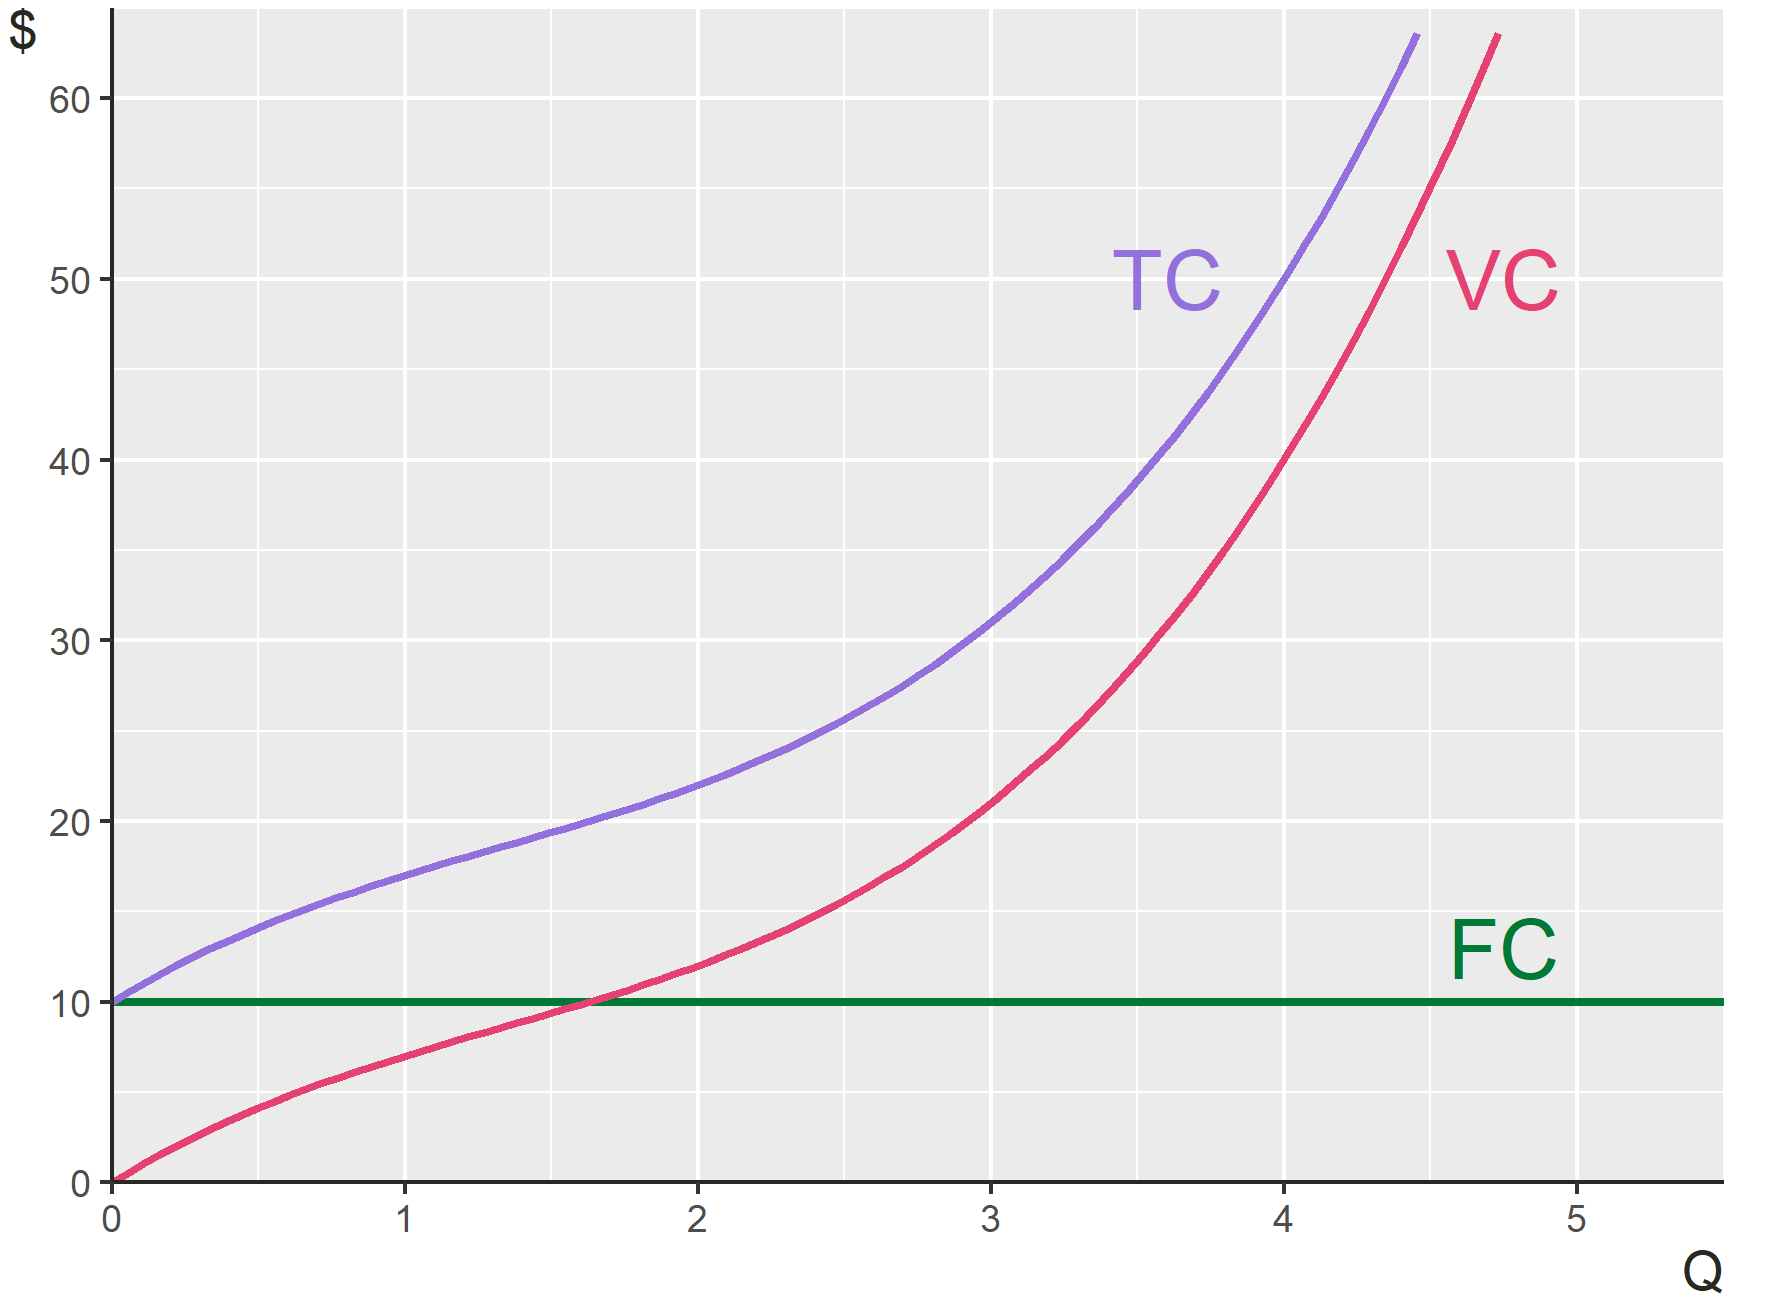
\includegraphics[width=7cm]{tc vc fc.png}
        \caption*{TC and VC are based on cubic equations, for reference}
    \end{figure}
\end{frame}

\begin{frame}{Typical AFC}
    \begin{itemize}[<+->]
        \item FC is constant, so AFC will look like $\frac{1}{x}$ (i.e. $\frac{1}{Q}$)\pause
        \begin{figure}
            \centering
            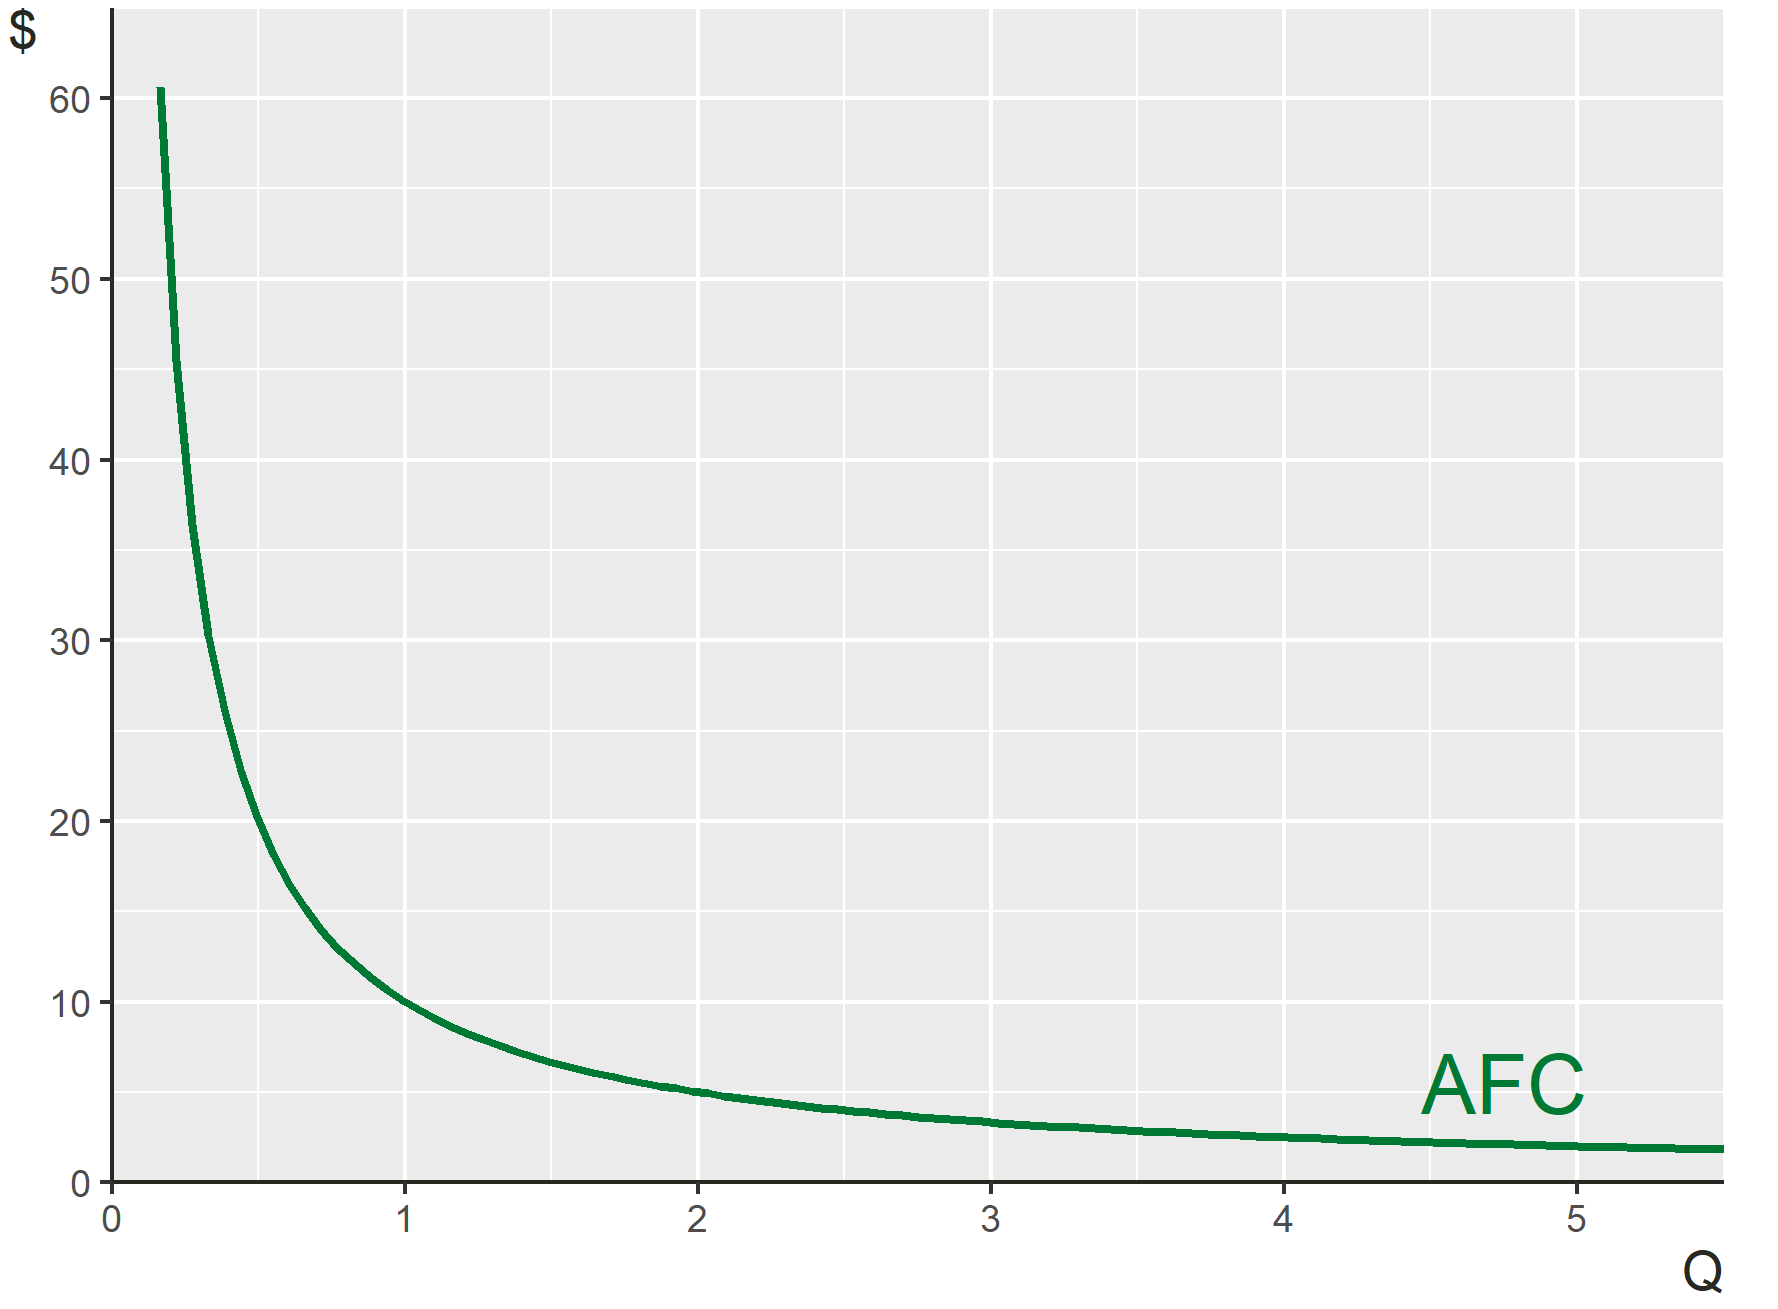
\includegraphics[width=7cm]{afc.png}
        \end{figure}
    \end{itemize}
\end{frame}

\begin{frame}{Typical ATC and AVC}
    \begin{itemize}[<+->]
        \item Note that since $TC=FC+VC$, dividing the whole equation by $Q$ implies \pause
        $$ATC=AFC+AVC$$
        \item Therefore, the height difference between ATC and AVC is equal to AFC
        \begin{figure}
            \centering
            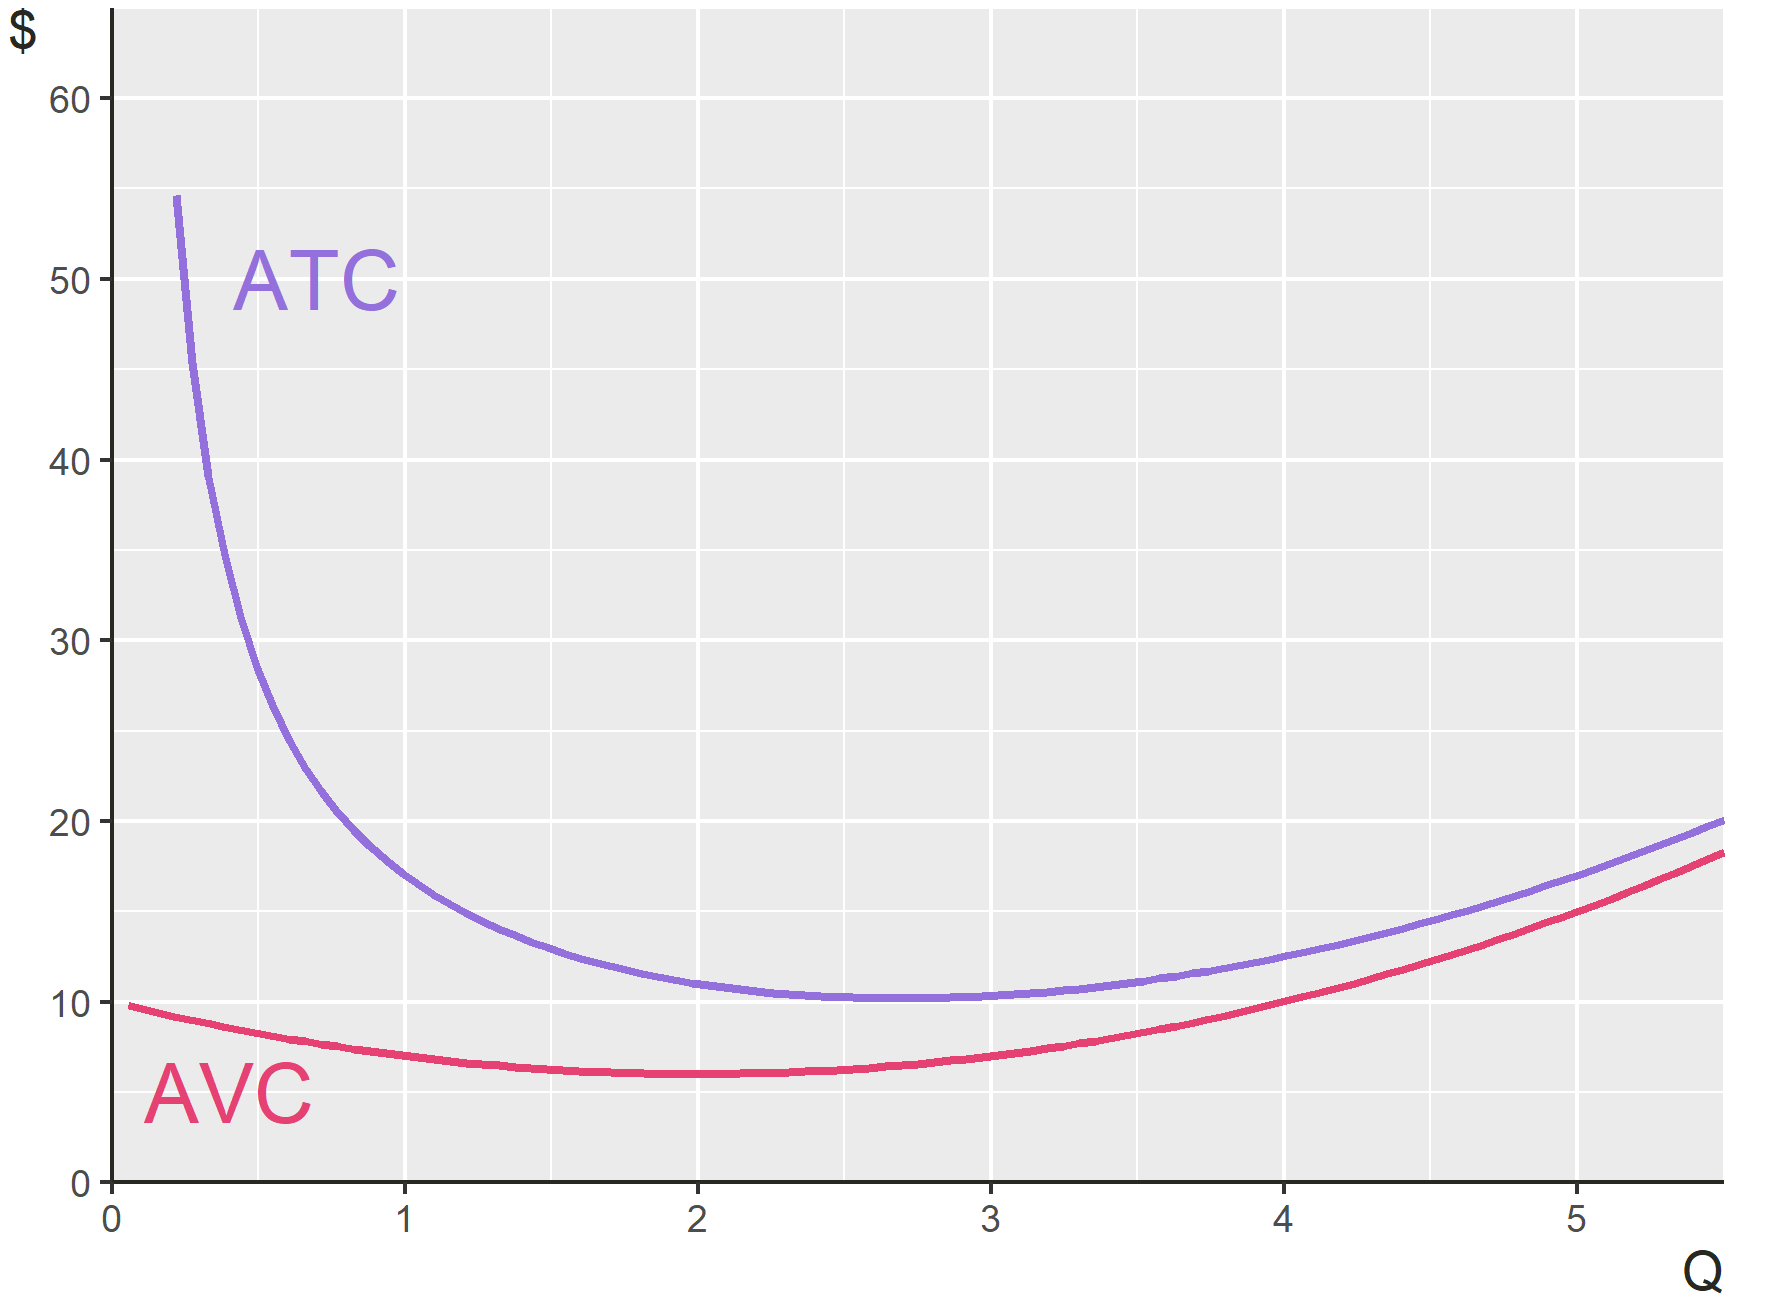
\includegraphics[width=7cm]{atc avc.png}
        \end{figure}
    \end{itemize}
\end{frame}

\begin{frame}{Typical ATC and AVC (cont.)}
    \begin{itemize}[<+->]
        \item Note that when VC is near 0, ATC looks like AFC. As fixed costs get stretched over more production (so that AFC$\to0$), our ATC tends towards and become AVC  
        \begin{figure}
            \centering
            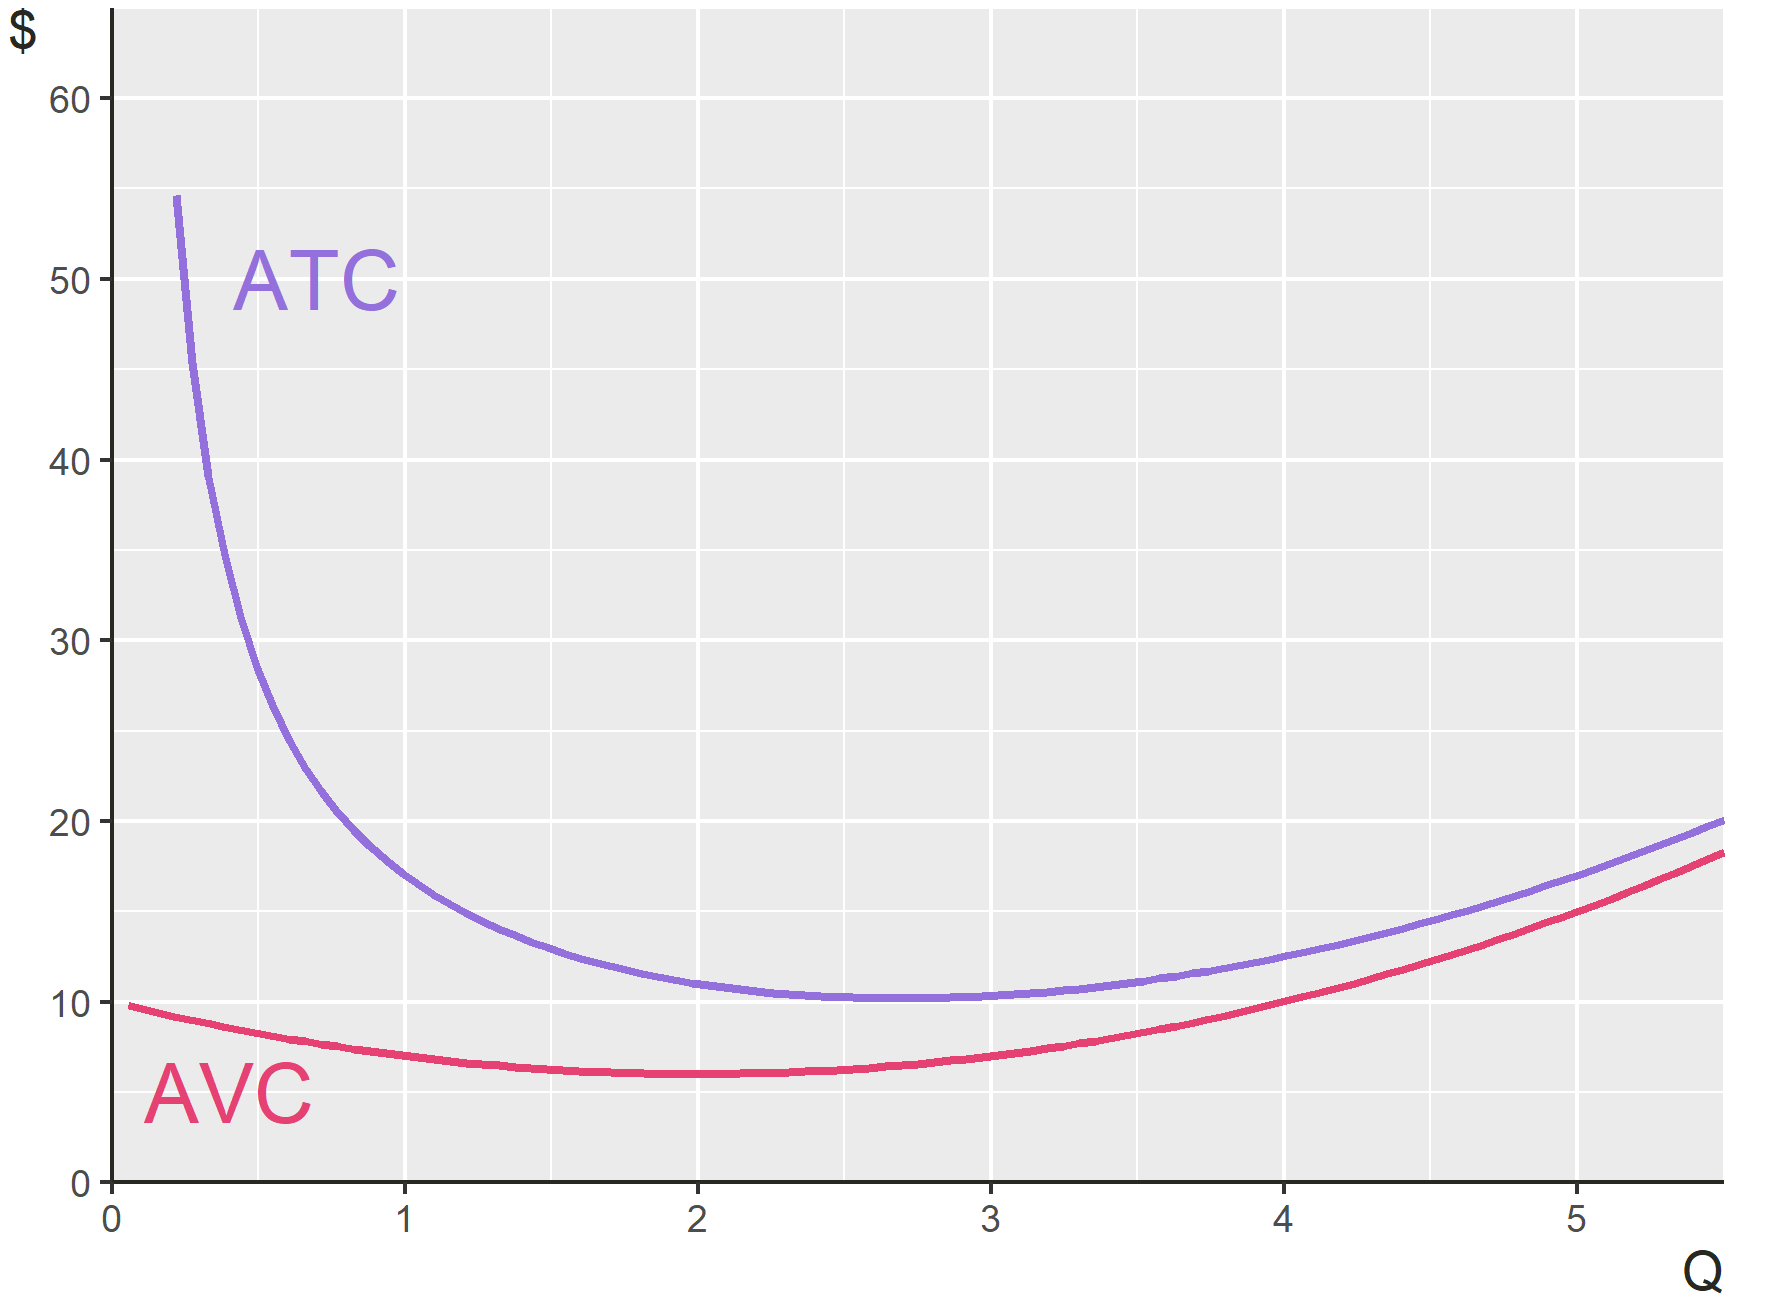
\includegraphics[width=6cm]{atc avc.png}
        \end{figure}
        \item With that important part said, we may, for shorthand, just draw ATC as a parabola floating above AVC
    \end{itemize}
\end{frame}

\begin{frame}{MC with ATC}
    \begin{itemize}[<+->]
        \item Finally, MC has a parabolic shape that often resembles a Nike swoosh
        \begin{figure}
            \centering
            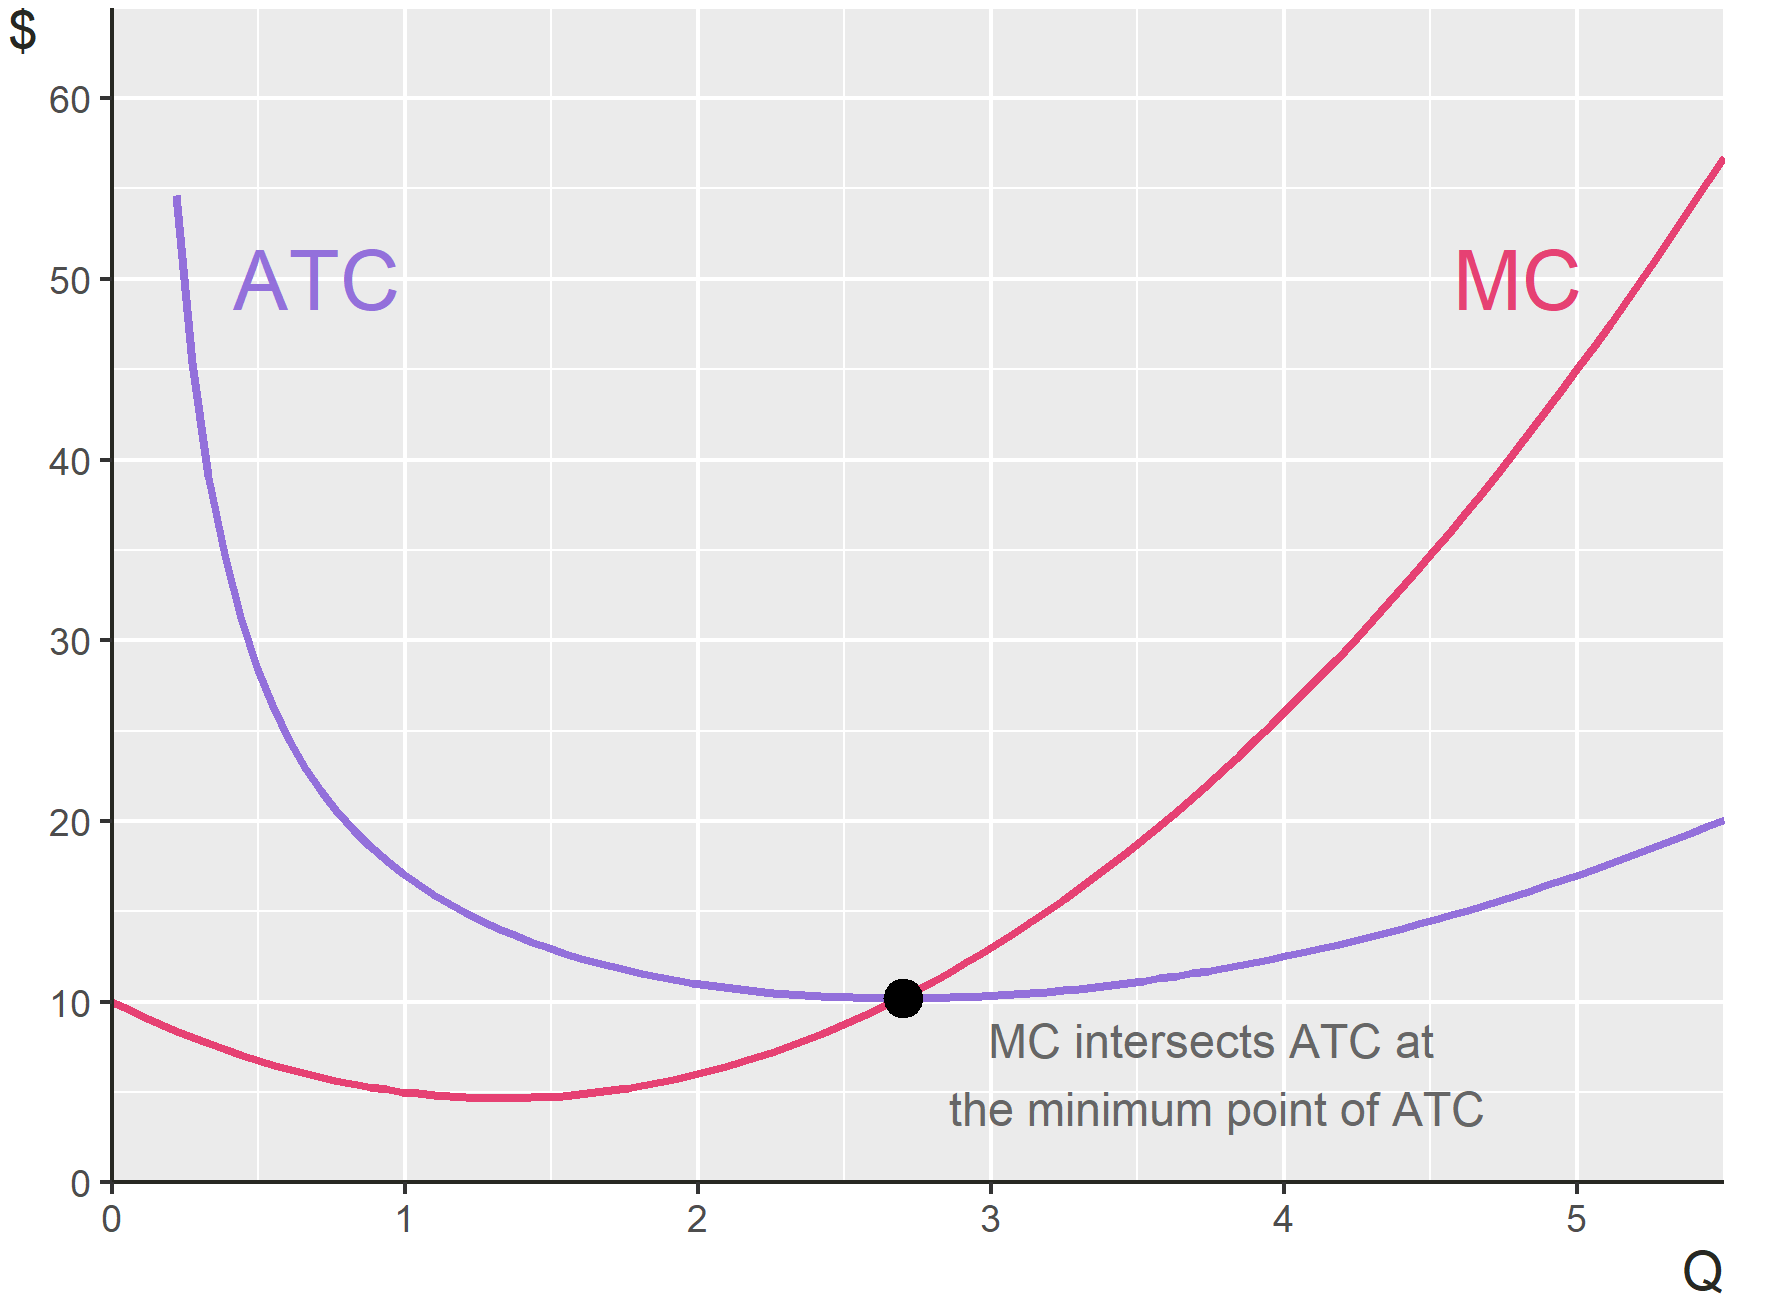
\includegraphics[width=7cm]{mc atc.png}
        \end{figure}
        \item Note that the MC curve \textbf{always} intersects ATC at the minimum ATC (this will be very important later)
    \end{itemize}
\end{frame}

\begin{frame}{Some Notes about these Curves}
    \begin{itemize}[<+->]
        \item Because MC crosses ATC at ATC's minimum, the following are true
        \begin{itemize}
            \item Whenever marginal cost is less than average total cost, average total cost is falling
            \item Whenever marginal cost is greater than average total cost, average total cost is rising
            \begin{itemize}
                \item Analogy: if your next (marginal) assignment grade is worse than your average grade in this class, your grade will go down. If it is better, your grade will go up
            \end{itemize}
        \end{itemize}
        \item 
    \end{itemize}
\end{frame}

\section*{Costs -- Time Horizon}

\begin{frame}{Short vs Long Run}
    \begin{itemize}[<+->]
        \item You may have heard economists use the terms short run and long run before
        \item Depending on context, these are notions that can mean different things
        \begin{itemize}
            \item In some contexts, for example, the distinction is with how sticky prices are: the short run is when prices do not move as much
            \item In this class, the distinction will mostly be defined by whether or not there are fixed costs
        \end{itemize}
    \end{itemize}
\end{frame}

\begin{frame}{Defining the Notion of Long Run}
    \begin{itemize}[<+->]
        \item Recall that fixed costs can ``sort of" depend on output: if the restaurant flips a million burgers, they have to replace their stove; if they flip 2 million, they will expand
        \item However, if a restaurant is thinking on the time horizon of selling a \textit{million} burgers, then fixed costs are drowned out by the large amount of production
        \item Therefore, our rough definition for the \underline{\textbf{long run}} will be that there are \textit{no fixed costs}
        \begin{itemize}
            \item Put another way: \textit{all inputs are variable in the long run}
            \item That is: factories can change their size, machines, and mode of production in the long run, but must keep some such factors fixed in the short run
        \end{itemize}
    \end{itemize}
\end{frame}

\begin{frame}{Deriving Long Run ATC}
    \begin{itemize}[<+->]
        \item A firm can choose from three factory sizes: small, medium, or large
        \item Each factory size has its own short-run ATC curve\pause
        \begin{figure}
            \centering
            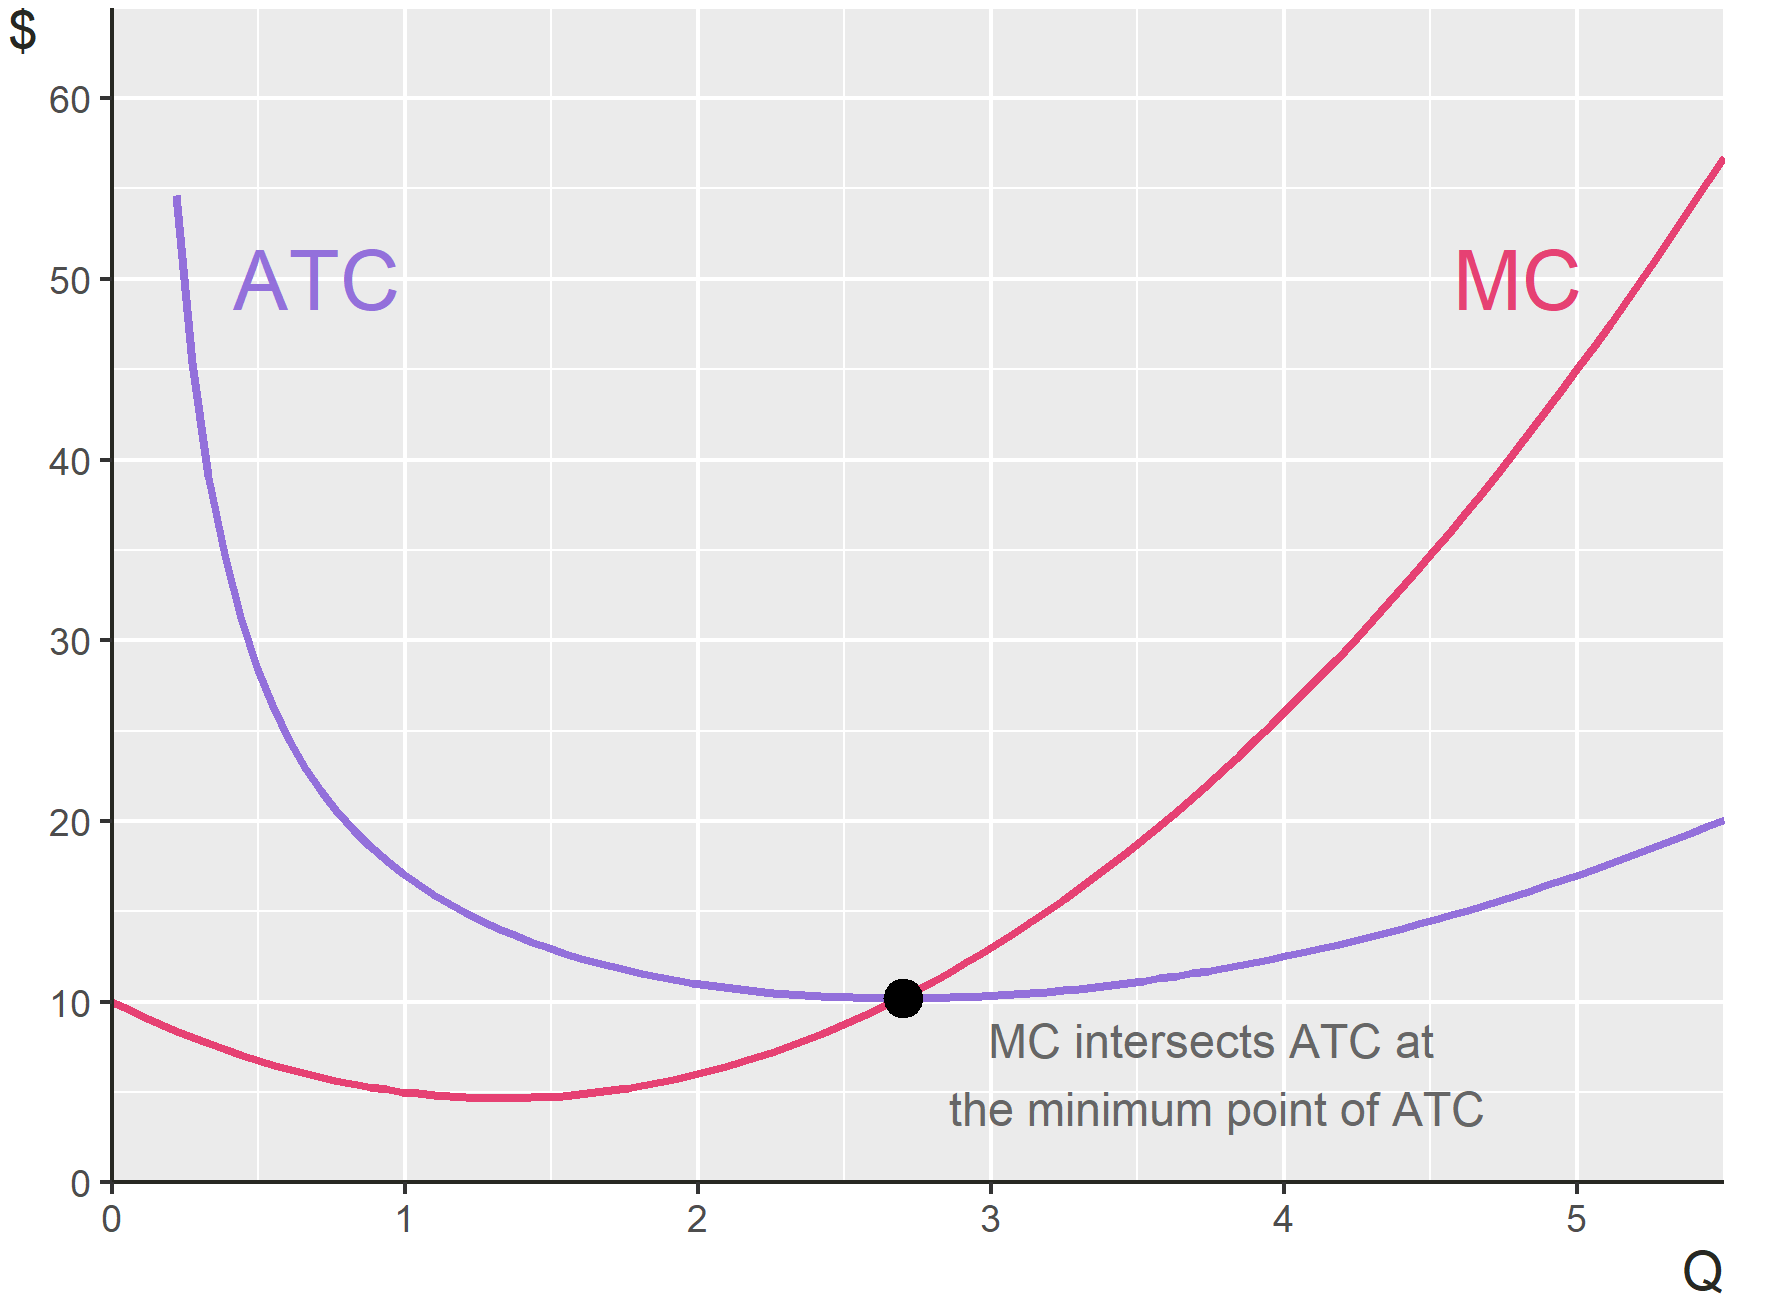
\includegraphics[width=7cm]{mc atc.png}
        \end{figure}
    \end{itemize}
\end{frame}

\begin{frame}{Deriving Long Run ATC (cont.)}
    \begin{itemize}[<+->]
        \item The firm can change to a different factory size in the long run, but not in the short run
        \begin{figure}
            \centering
            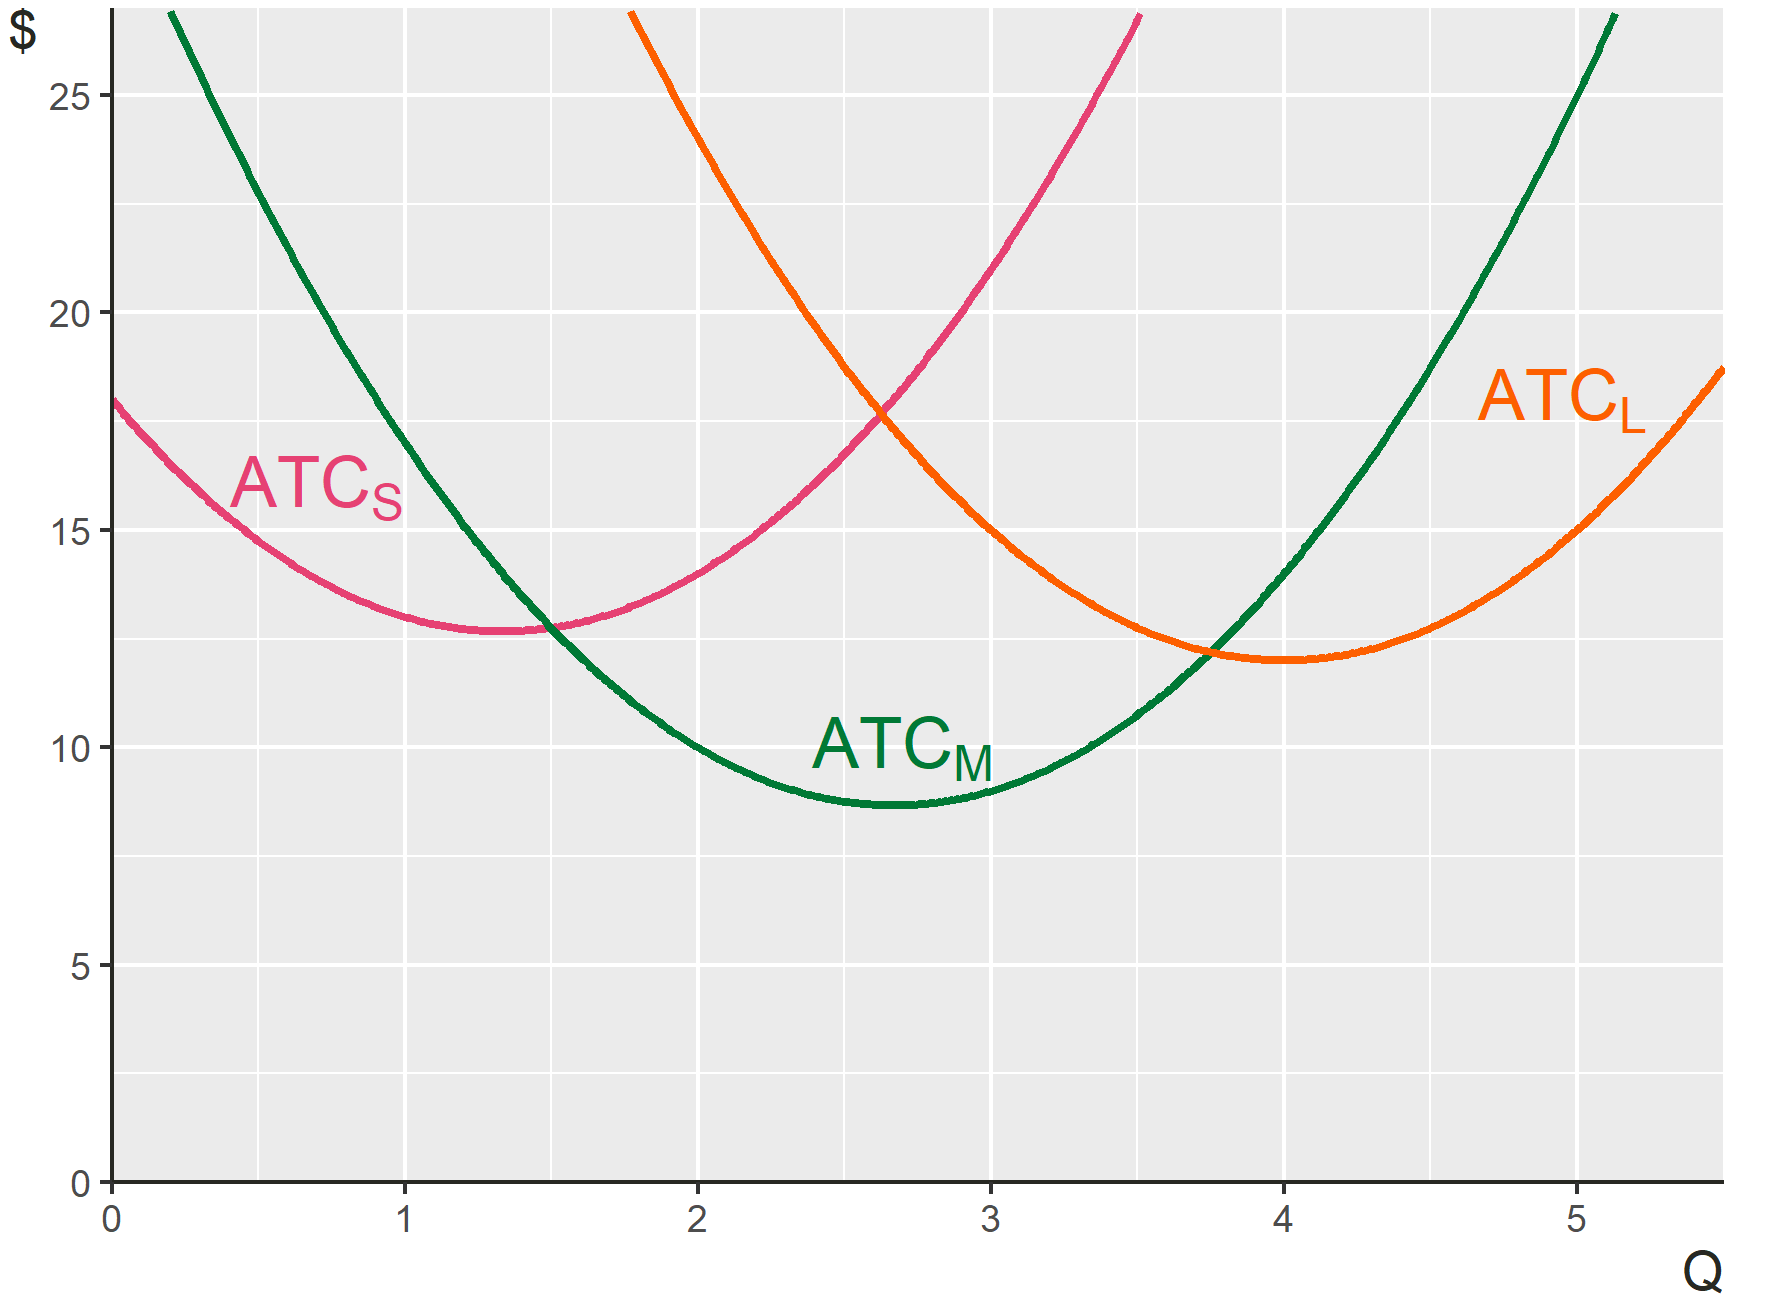
\includegraphics[width=7cm]{3 atcs.png}
        \end{figure}
        \item What will the firm do in the long run?
    \end{itemize}
\end{frame}

\begin{frame}{Deriving Long Run ATC (cont.)}
    \begin{itemize}[<+->]
        \item In the long run, the firm will do whatever is the cheapest option, since they have full flexibility in their scale
        \item Hence, the \underline{Long Run Average Total Cost} (LRATC) in this example is shown by
        \begin{figure}
            \centering
            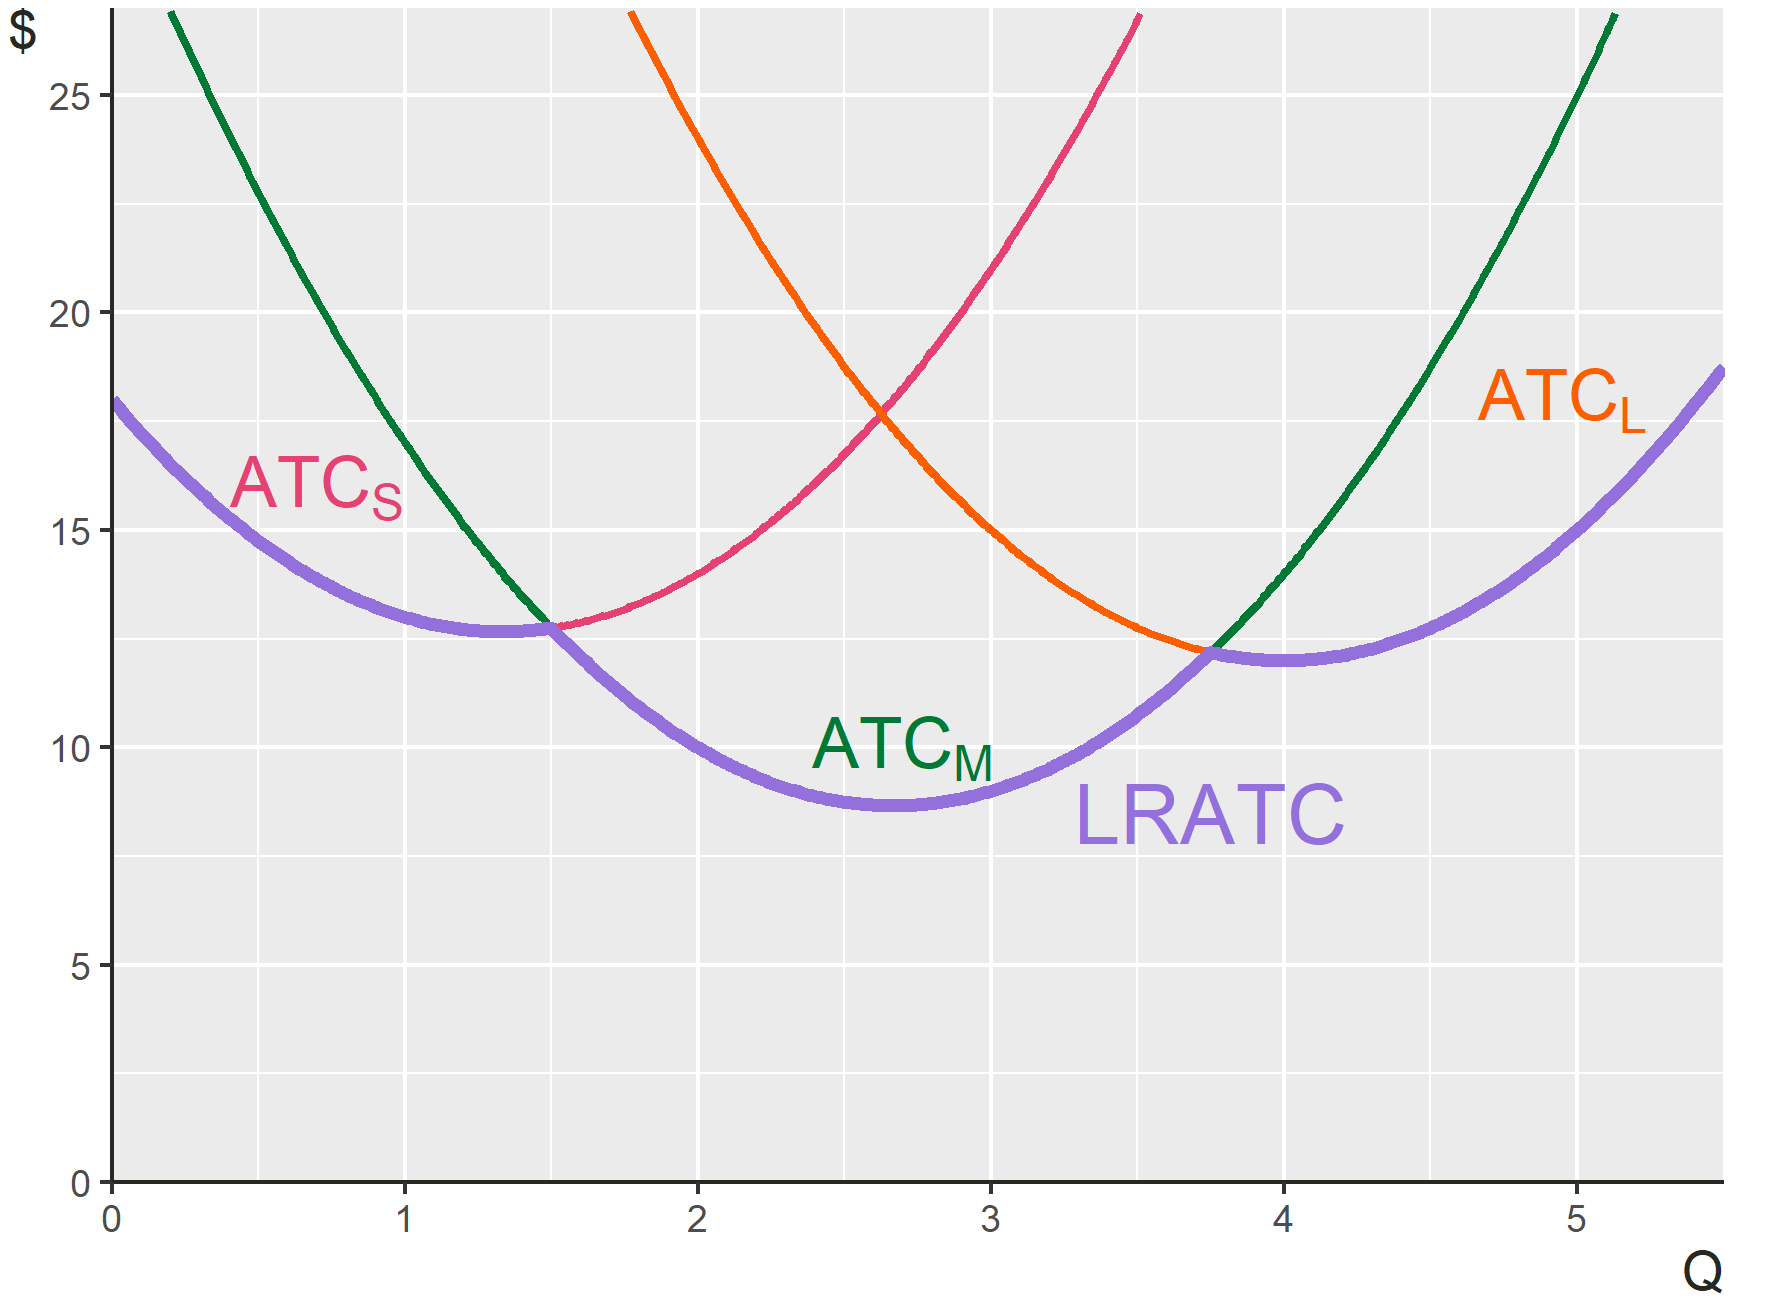
\includegraphics[width=7cm]{atcs lratc.png}
        \end{figure}
    \end{itemize}
\end{frame}

\begin{frame}{Typical LRATC}
    \begin{itemize}[<+->]
        \item When considering a lot of different sizes over a lot of different production levels, we get a typical LRATC
        \begin{figure}
            \centering
            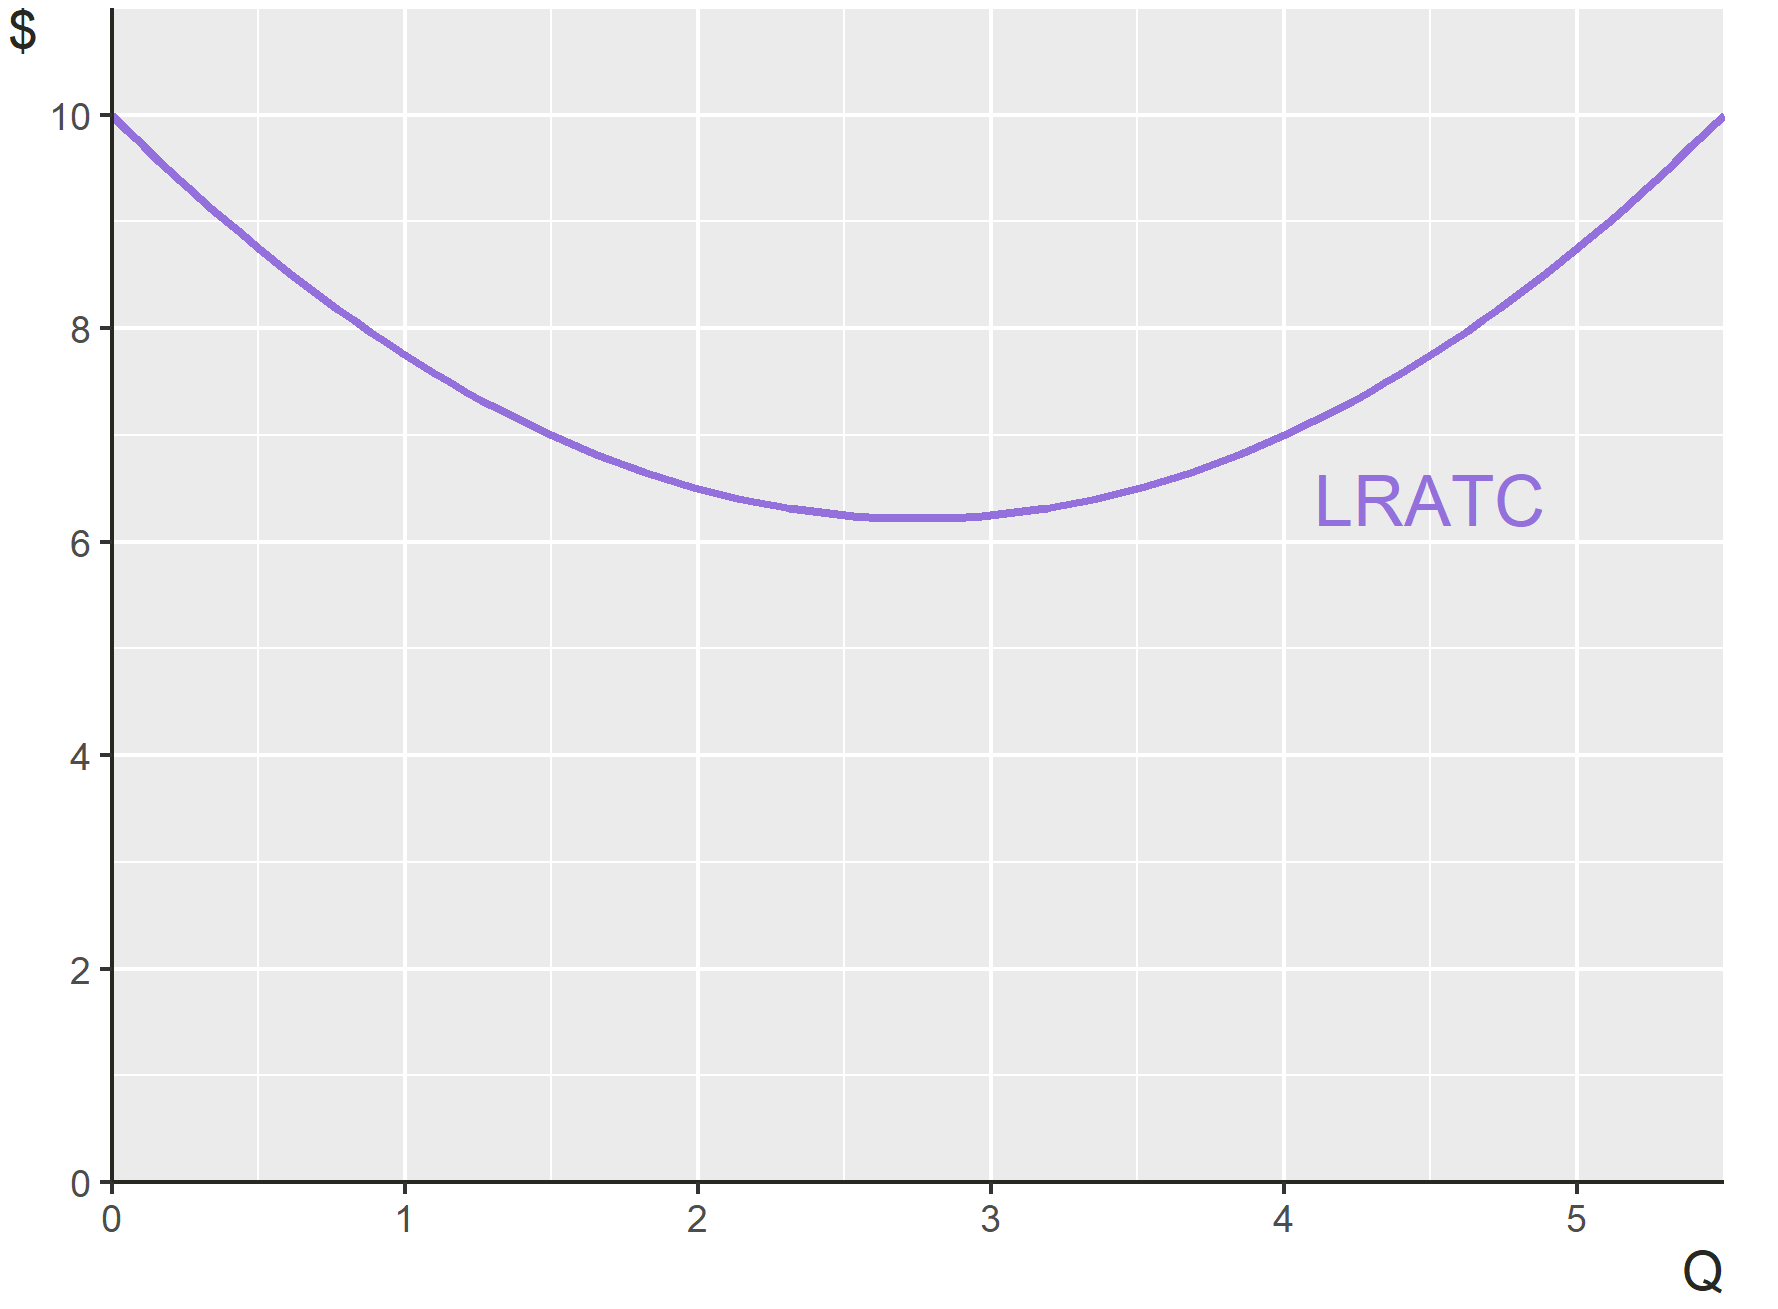
\includegraphics[width=7cm]{lratc.png}
        \end{figure}
        \item There is often variation in how you can draw this, due to what we call \textit{returns to scale} (RTS)
    \end{itemize}
\end{frame}

\begin{frame}{Returns to Scale}
    \begin{itemize}[<+->]
        \item Returns to scale measures the qualitative slope of LRATC, as output changes
            \begin{itemize}
                \item That is: as we increase output (in the long run), are costs getting more expensive, less expensive, or about equal
                \item Remember the relationship between a cost function and a production function: this is often a story of the state of the production function
            \end{itemize}
    \end{itemize}
\end{frame}

\begin{frame}{Another Typical LRATC}
        \begin{figure}
            \centering
            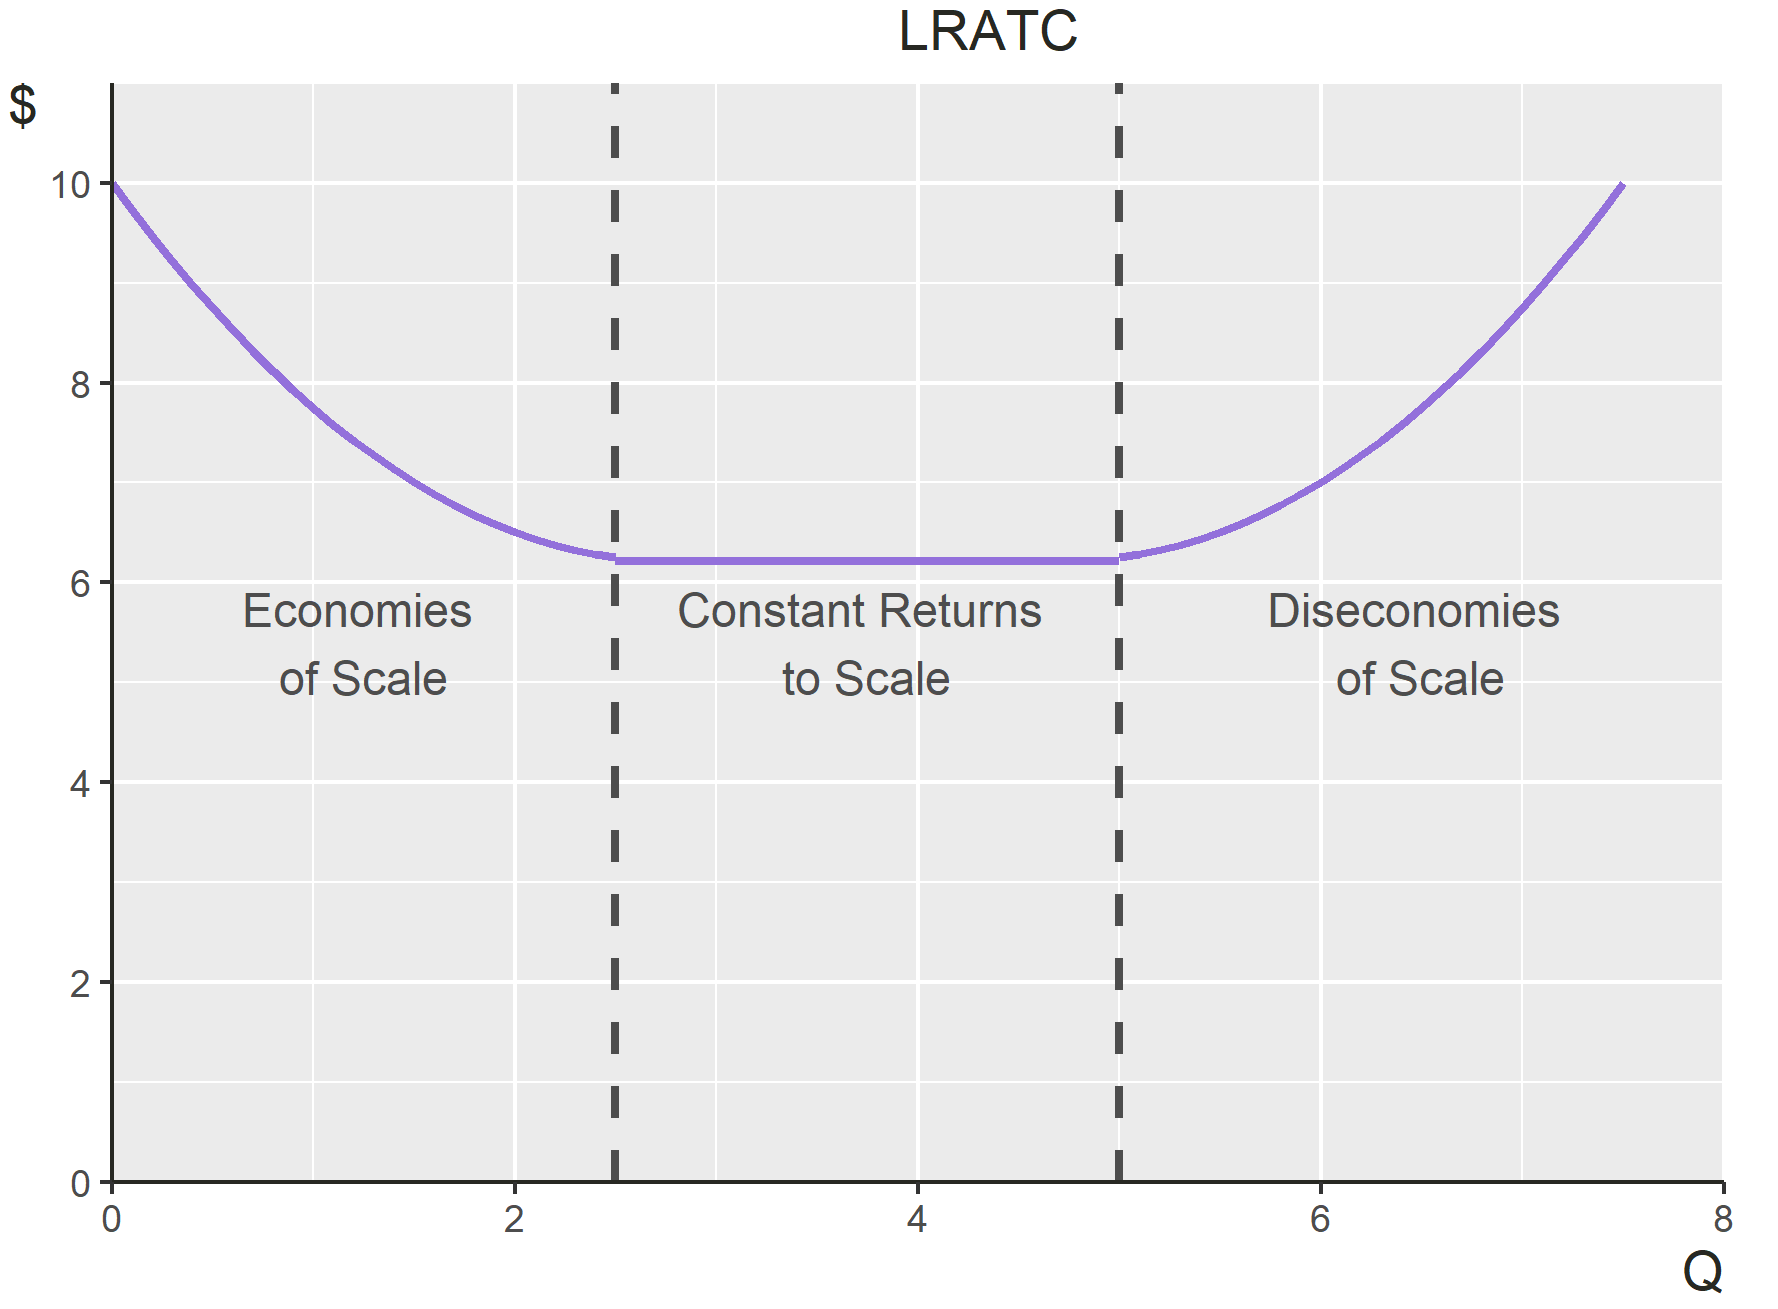
\includegraphics[width=8cm]{longer lratc.png}
        \end{figure}
\end{frame}

\begin{frame}{Returns to Scale -- Definitions}
    \begin{enumerate}[<+->]
        \item \underline{\textbf{Economies of Scale}} (Positive RTS)
        \begin{itemize}
            \item Long-run ATC falls as the quantity of output rises
            \begin{itemize}
                \item Characterized by increased specialization in workers
                \item More common when $Q$ is low
                \item Ex: tech start-ups
            \end{itemize}
        \end{itemize}
        \item \underline{\textbf{Constant Returns to Scale}}
        \begin{itemize}
            \item Long-run ATC stays the same as the quantity of output rises
            \begin{itemize}
                \item What you get in is what you get out
                \item Ex: restaurant chains
            \end{itemize}
        \end{itemize}
        \item \underline{\textbf{Diseconomies of Scale}} (Negative RTS)
        \begin{itemize}
            \item Long-run ATC rises as the quantity of output rises
            \begin{itemize}
                \item It is costly to keep expanding 
                \item Coordination problems in large firms
                \item More common when $Q$ is high
                \item Ex: McDonald's origin -- as restaurants expand, you can't manage quality
            \end{itemize}
        \end{itemize}        
    \end{enumerate}
    \begin{itemize}
        \item We will return to the notion of short versus long run later, under the context of supply curves
    \end{itemize}
\end{frame}


\section*{Perfectly Competitive Markets}

\begin{frame}{Types of Firms}
    \begin{itemize}[<+->]
        \item So far, we have only talked about the breakdown of costs that a firm faces, but not \textit{why} we care about them and what we should do with them
        \item In general, how a firm turns cost structure into supply decisions depends on the relative market power of a firm:
        \begin{itemize}
            \item If costs go up for a firm like Comcast, they can likely pass those costs onto consumers, much easier than an Amazon seller
        \end{itemize}
        \item In general, we break down the types of firms into the following picture\footnote{Anything other than perfect competition is refereed to as \textit{imperfect competition}}:
        \begin{figure}
            \centering
            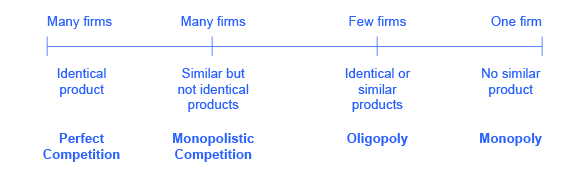
\includegraphics[width=10cm]{comp market specturm.jpg}
        \end{figure}
    \end{itemize}
\end{frame}

\begin{frame}{Ends of the Spectrum}
    \begin{itemize}[<+->]
        \item In this class, we will talk in detail only about the ends of this spectrum: perfect competition (PC) and pure monopoly
        \begin{itemize}
            \item We will start with PC and then move to monopoly
            \item Once we have these key ideas down, the qualitative parts of monopolistic competition and oligopoly will be straightforward to see, and the more numerical parts require calculus
        \end{itemize}
        \item What is the most important decision that you think these firms make, once they have their costs, and know how much they are going to produce?
            \begin{itemize}
                \item How much they are going to sell for -- i.e., price
            \end{itemize}
        \item In terms of price, firms in perfect competition and monopoly are respectively refereed to as \textit{price takers} and \textit{price makers}
    \end{itemize}
\end{frame}

\begin{frame}{Key Descriptors to a PC Market}
    \begin{itemize}[<+->]
        \item The key descriptors of a perfectly competitive market are as follows:
        \begin{enumerate}
            \item Many buyers and sellers in the market
            \item Near-identical products being sold
        \end{enumerate}
        With a third key descriptor, which we will often relax \footnote{i.e., we may do PC examples where it does not hold}
        \begin{enumerate}
            \item[3.] Free entry and exit
        \end{enumerate}
        \item Here are some examples:
        \begin{itemize}
            \item Rice bracelets in Latin-American countries: many street vendors selling near-identical rice bracelets at near identical prices
            \item Amazon sellers: many vendors selling knock-offs of the same product for similar prices (this might be more of monopolistic competition, but again, our examples will be relaxed)
            \item Agriculture: many farmers selling similar crops who have no individual say in the price of those crops (point 3 may not be satisfied here)
        \end{itemize}
    \end{itemize}
\end{frame}

\begin{frame}{Firms as Price Takers}
    \begin{itemize}[<+->]
        \item What do these firms have in common? 
        \begin{itemize}
            \item They have little individual say in what happens to the price of the good they are selling
            \item For instance, if a particular farmer or bracelet seller is hit with an individual hardship, if they raise the price, then the market drops out
        \end{itemize}
        \item Therefore, these firms are regarded as \textit{price takers}, which is another key phrase to describe perfectly competitive firms\footnote{The other three are the ``officially descriptors, this description just follows form the others"}
        \item In other words, in this section, price will just \textit{fall out of the sky} for the firms, and they will take it as given
        \item Again, if a firm raises it's price, they lose the whole market
        \item What do you think happens if the firm tries to lower the price?
        \begin{itemize}
            \item They will gain the whole market, but their production will increase to a level such that they lose profit
        \end{itemize}
    \end{itemize}
\end{frame}

\begin{frame}{How Firms Choose Production Decisions}
    \begin{itemize}[<+->]
        \item Therefore, for the PC firm, the only decision they need to make in order to maximize profit is how much to produce
        \item Recall the thinking for finding the optimal number of workers to hire:\pause if it's profitable to keep going, keep going; if we are losing profit, go back; if we break even, we are at the sweet spot
        \item A firm trying to maximize profit will do the same thing: if it's worth it to sell another unit it, do it; if it's not, don't
        \begin{itemize}
            \item Therefore, a firm will produce another unit if the revenue it makes from selling another unit exceeds the cost of selling that unit
            \item In other words, the firm will produce another unit as long as \textit{marginal revenue} exceeds \textit{marginal cost}
        \end{itemize}
        \item[$\bigstar$] Following the motivation above, the firm (\textit{any firm}) produces another unit up until
        $$\boxed{MR=MC}$$
        \item This is the general optimality condition for a firm choosing how much to produce
    \end{itemize}
\end{frame}

\begin{frame}{Optimally Producing Firm}
    \begin{itemize}[<+->]
        \item Given the following information, where does a firm produce at?
        \begin{table}[H]
            \centering
            \begin{tabular}{c|c|c|c|c|c|c}
                \thead{\textbf{Output}} & 
                \thead{\textbf{TR}} & 
                \thead{\textbf{TC}} & 
                \thead{$\pi$} & 
                \thead{\textbf{MR}} &
                \thead{\textbf{MC}} & 
                \thead{$\Delta \pi$} \\ 
                \hline
                0 & 0 & 20 & -20 & {--} & {--} & {--} \\
                \hline
                1 & 24 & 22 &  &  &  &  \\
                \hline
                2 & 48 & 28 &  &  &  & \\
                \hline
                3 & 72 & 38 &  &  &  & \\
                \hline
                4 & 96 & 52 &  &  &  & \\
                \hline
                5 & 120 & 70 &  &  &  & \\
                \hline
                6 & 144 & 92 &  &  &  & \\
                \hline
                7 & 168 & 118 &  &  &  & \\
                \hline
                8 & 192 & 148 &  &  &  & \\
                \end{tabular}
        \end{table}
        \item Note: filling out this table on your own is good practice, but we only need to fill out the MR and MC columns to answer this question!
    \end{itemize}
\end{frame}

\begin{frame}{Optimally Producing Firm}
    \begin{itemize}[<+->]
        \item Note: filling out this table on your own is good practice, but we only need to fill out the MR and MC columns to answer this question!\footnote{I started on the other columns, just to help with the additional question}
        \begin{table}[H]
            \centering
            \begin{tabular}{c|c|c|c|c|c|c}
                \thead{\textbf{Output}} & 
                \thead{\textbf{TR}} & 
                \thead{\textbf{TC}} & 
                \thead{$\pi$} & 
                \thead{\textbf{MR}} &
                \thead{\textbf{MC}} & 
                \thead{$\Delta \pi$} \\ 
                \hline
                0 & 0 & 18 & -18 & {--} & {--} & {--} \\
                \hline
                1 & 24 & 22 & 2 & 24 & 4 & 20 \\
                \hline
                2 & 48 & 30 & 18 & 24 & 8 & 16\\
                \hline
                3 & 72 & 42 & 30 & 24 & 12 & 12\\
                \hline
                4 & 96 & 48 &  & 24 & 16 & \\
                \hline
                5 & 120 & 58 &  & 24 & 20 & \\
                \hline
                6 & 144 & 82 &  & \tr{24} & \tr{24} & \\
                \hline
                7 & 168 & 110 &  & 24 & 28 & \\
                \hline
                8 & 192 & 142 &  & 24 & 32 & \\
                \end{tabular}
        \end{table}
        \item Particularly, if you fill out $\Delta \pi$, what do you see as we approach and go through $Q=6$?
    \end{itemize}
\end{frame}

\begin{frame}{Marginal Revenue}
    \begin{itemize}[<+->]
        \item Recall that total revenue for a firm is given by $TR=P\cdot Q$
        \item Define \underline{\textbf{Marginal Revenue}} for the firm as the change in TR from selling one additional unit,
        where $\Delta Q$ is usually equal to 1
        \item Since price is fixed and falls from the sky (in a PC market), and selling an additional unit just gives you revenue equal to the price of that unit, we get the following result for a PC firm
        $$\boxed{MR=P}$$
        \item That is, marginal revenue is constant and equal to price
        \vspace{2mm}
        \item Note: when a larger firm has influence over it's price, selling another unit might mean changing the price you are selling all units at, so this result is unique to PC markets
    \end{itemize}
\end{frame}


\begin{frame}{How Firms Choose Production Decisions}
    \begin{itemize}[<+->]
        \item Combing the general optimality rule for how much a firm should produce, $MR=MC$, with the PC firm's marginal revenue that was just derived, we get the following formula for where a PC firm should produce:
        $$\boxed{P=MC}$$
        \item Verbally, a firm should produce such that marginal cost is equal to the price
    \end{itemize}
\end{frame}

\begin{frame}{Optimally Producing PC Firm}
    \begin{itemize}[<+->]
        \item Given the following information, where does a PC firm produce at?
        \begin{table}[H]
            \centering
            \begin{tabular}{c|c|c|c|c|c|c|c}
                \thead{\textbf{Output}} & 
                \thead{\textbf{P}} & 
                \thead{\textbf{TR}} & 
                \thead{\textbf{TC}} & 
                \thead{$\pi$} & 
                \thead{\textbf{MR}} &
                \thead{\textbf{MC}} & 
                \thead{$\Delta \pi$} \\ 
                \hline
                0 & 6 &  & 8 &  & {--} & {--} & {--}\\
                \hline
                1 & 6 &  & 9 &  &  &  & \\
                \hline
                2 & 6 &  & 12 &  &  & & \\
                \hline
                3 & 6 &  & 17 &  &  & & \\
                \hline
                4 & 6 &  & 24 &  &  & & \\
                \hline
                5 & 6 &  & 33 &  &  & & \\
                \hline
                6 & 6 &  & 44 &  &  & & \\
                \hline
                7 & 6 &  & 57 &  &  & & \\
                \hline
                8 & 6 &  & 72 &  &  & &\\
                \end{tabular}
        \end{table}
    \end{itemize}
\end{frame}

\begin{frame}{Optimally Producing PC Firm}
    \begin{itemize}[<+->]
        \item Note: filling out this table on your own is good practice, but we only need to fill out the MC column to answer this question!
            \begin{table}[H]
            \centering
            \begin{tabular}{c|c|c|c|c|c|c|c}
                \thead{\textbf{Output}} & 
                \thead{\textbf{P}} & 
                \thead{\textbf{TR}} & 
                \thead{\textbf{TC}} & 
                \thead{$\pi$} & 
                \thead{\textbf{MR}} &
                \thead{\textbf{MC}} & 
                \thead{$\Delta \pi$} \\ 
                \hline
                0 & 9 &  & 8 &  & {--} & {--} & {--}\\
                \hline
                1 & 9 &  & 9 &  &  & 1 & \\
                \hline
                2 & 9 &  & 12 &  &  & 3  & \\
                \hline
                3 & 9 &  & 17 &  &  & 5 & \\
                \hline
                4 & 9 &  & 24 &  &  & 7 & \\
                \hline
                5 & 9 &  & 33 &  &  & 9 & \\
                \hline
                6 & 9 &  & 44 &  &  & 11 & \\
                \hline
                7 & 9 &  & 57 &  &  & 13 & \\
                \hline
                8 & 9 &  & 72 &  &  & 15 &\\
                \end{tabular}
        \end{table}
        \item Bonus Question: How much profit does the firm make at this point?\pause\footnote{A: $\$12$}
    \end{itemize}
\end{frame}


\begin{frame}{Another Way to Write Profit}
    \begin{itemize}[<+->]
        \item Recall that profit for the firm is given by $\pi=TR-TC$
        \item Since $TR=P\cdot Q$, we can write this as
        $$\pi=PQ-TC$$
        \item Dividing by $Q$, we get
        $$\pi=(P-ATC)Q$$
        \item Assuming $Q>0$ (the firm is producing something), what does this say?
        \begin{itemize}
            \item $P>ATC\implies \pi>0$
            \item $P=ATC\implies \pi=0$
            \item $P<ATC\implies \pi<0$
        \end{itemize}
    \end{itemize}
\end{frame}


\begin{frame}{Visualizing Profit for a PC Firm}
    \begin{itemize}[<+->]
        \item Recall our example picture, now with price added:
        \begin{figure}
            \centering
            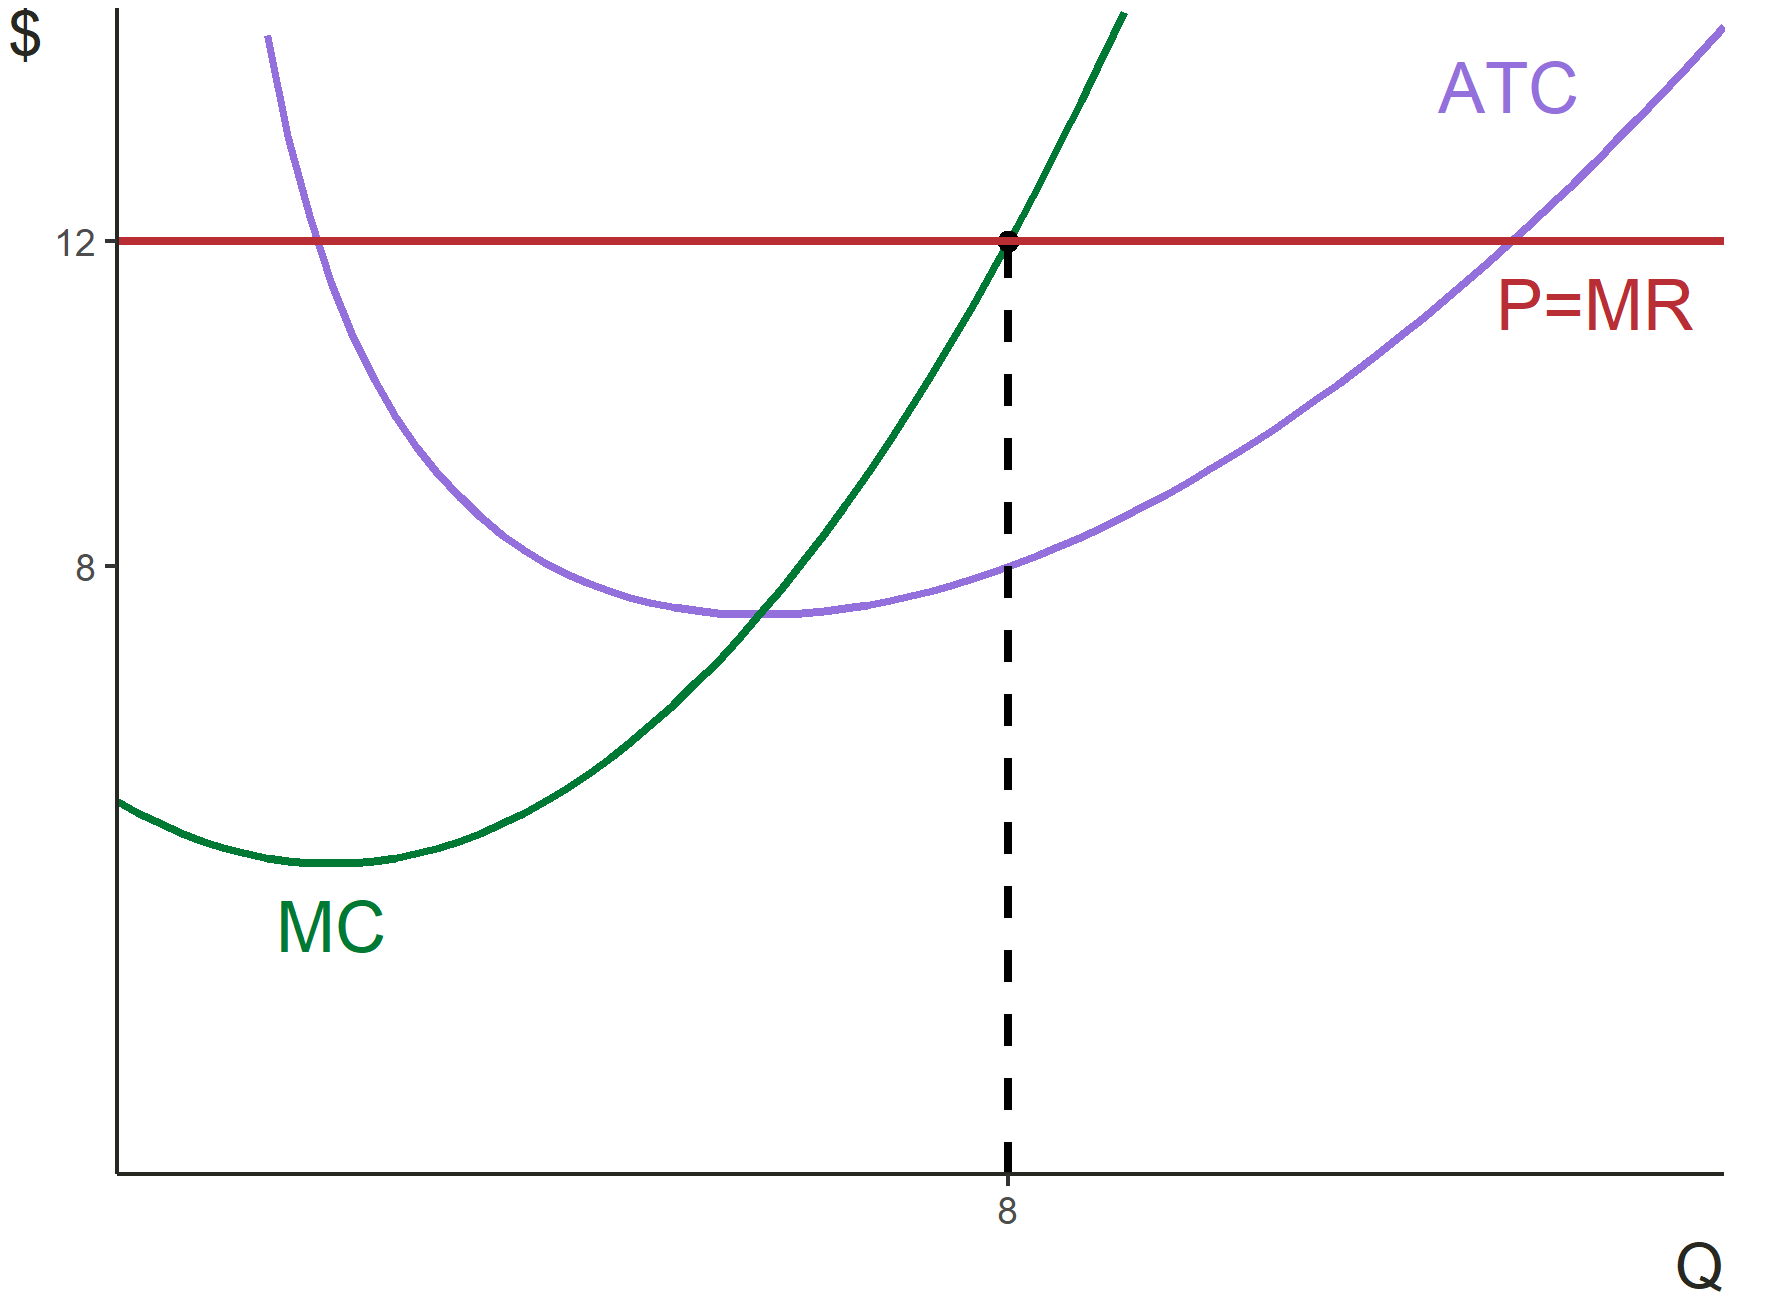
\includegraphics[width=8cm]{prod dec 1.png}
            \caption*{Note that the firm is choosing to produce where P=MC}
        \end{figure}
    \end{itemize}
\end{frame}

\begin{frame}{Visualizing Positive Profit for a PC Firm}
    \begin{itemize}[<+->]
        \item Since $\pi=(P-ATC)Q$, profit is given by the following box 
        \begin{figure}
            \centering
            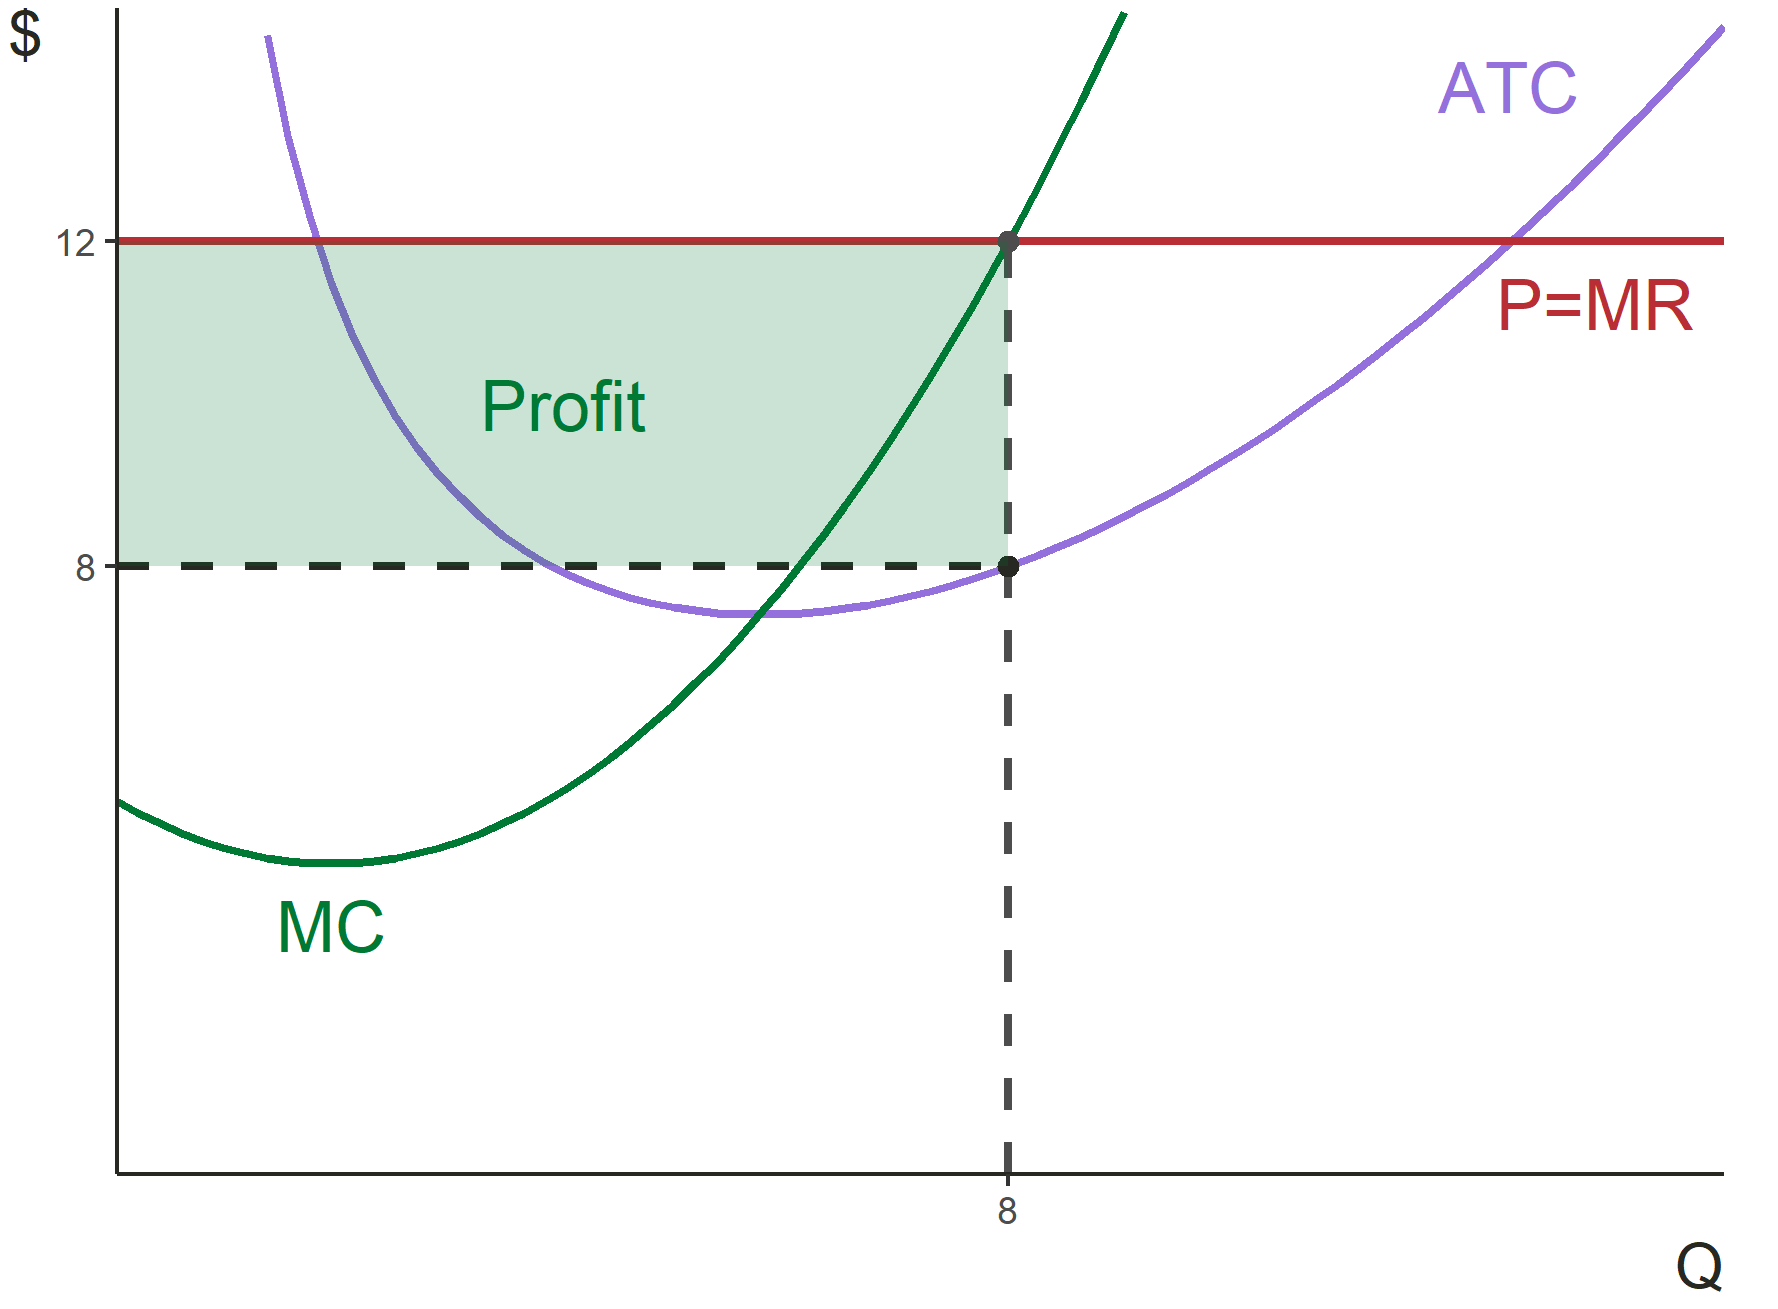
\includegraphics[width=8cm]{pmax1.png}
            \caption*{In this case, $\pi=8(12-8)=\$32$}
        \end{figure}
    \end{itemize}
\end{frame}

\begin{frame}{Visualizing Zero Profit for a PC Firm}
    \begin{itemize}[<+->]
        \item In this case, we produce at $P=MC$, and this induces $ATC$ to equal $P$, so we get a profit of 0: 
        \begin{figure}
            \centering
            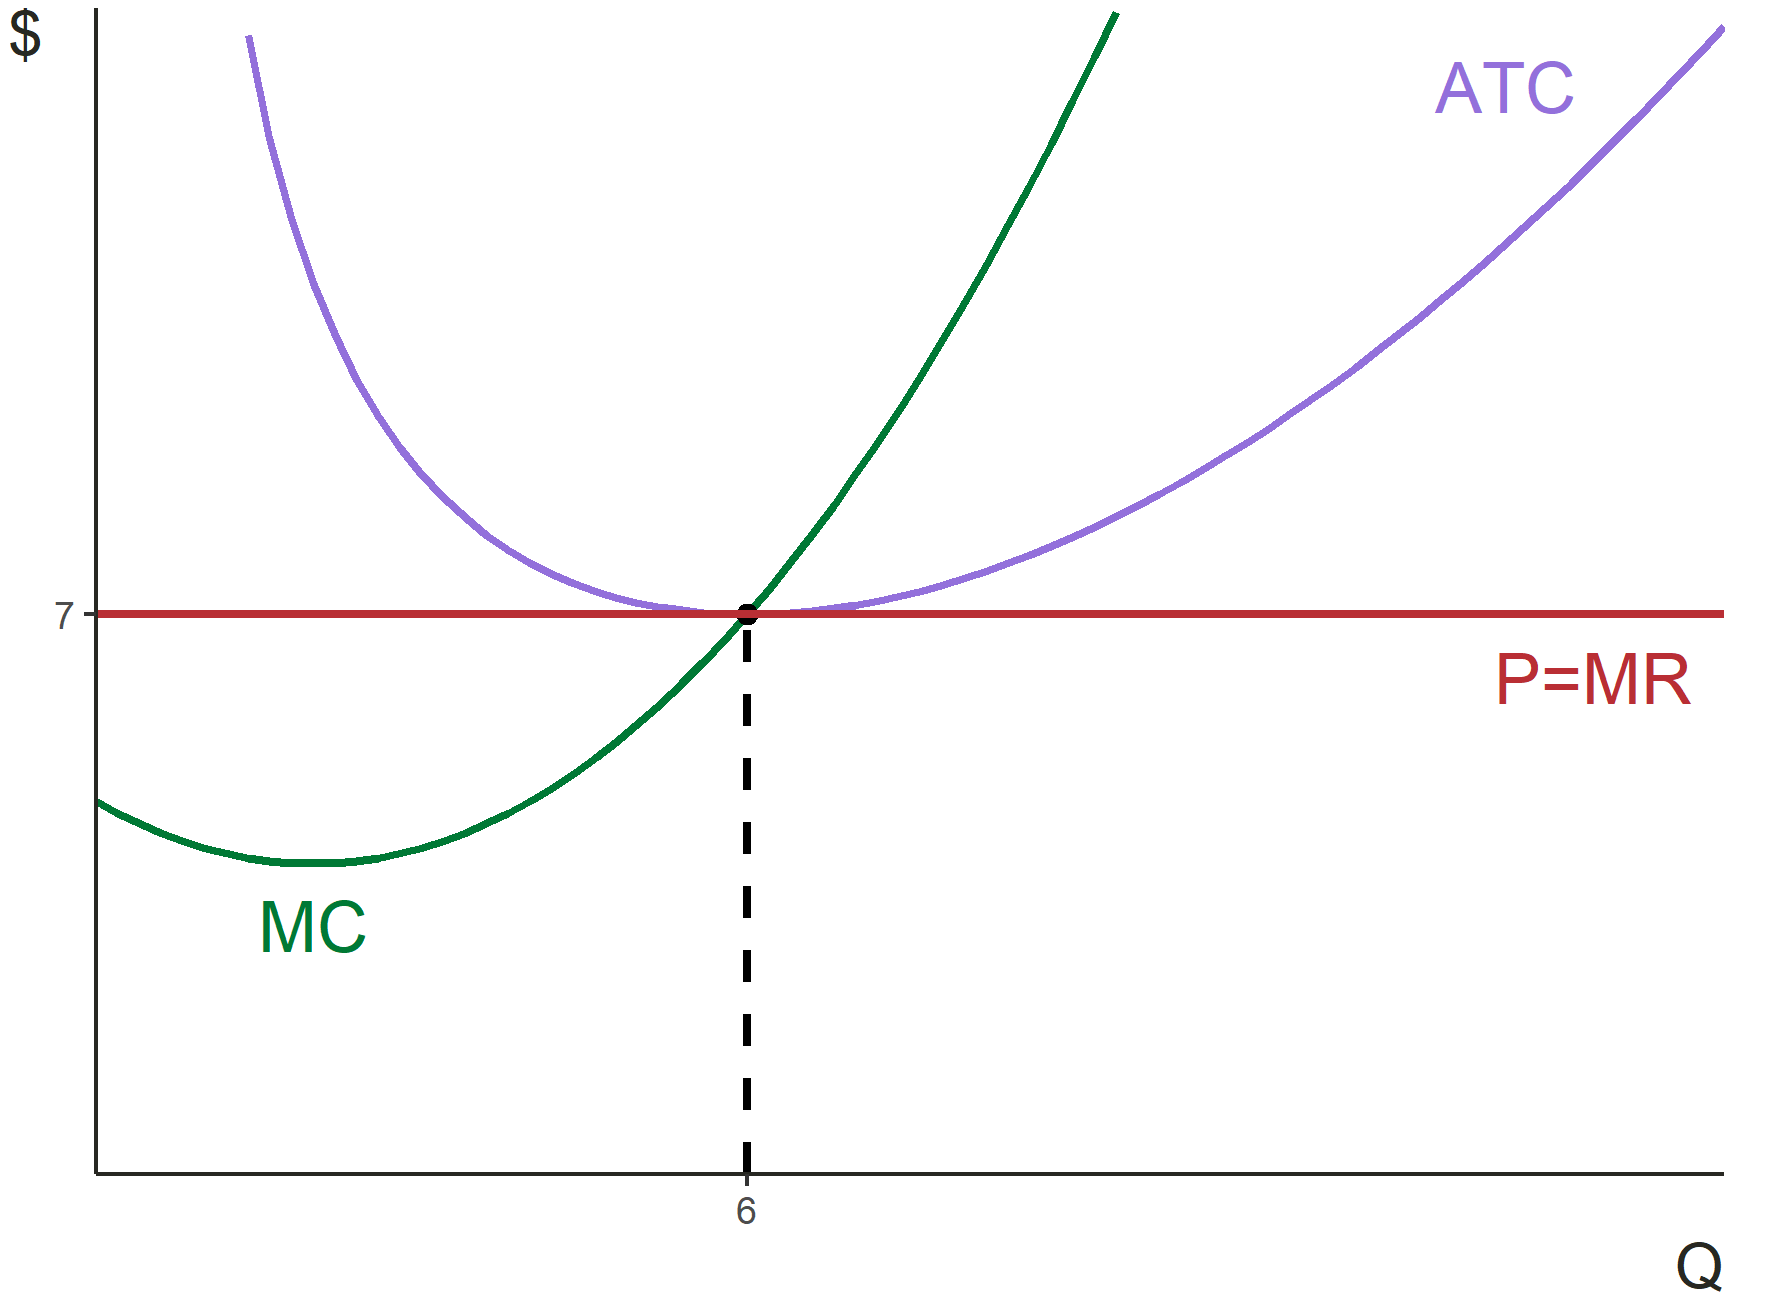
\includegraphics[width=8cm]{pmax2.png}
        \end{figure}
    \end{itemize}
\end{frame}

\begin{frame}{Visualizing Negative Profit for a PC Firm}
    \begin{itemize}[<+->]
        \item In this case, we produce at $P=MC$, and this induces $ATC$ to be below $P$, so we will make negative profit: 
        \begin{figure}
            \centering
            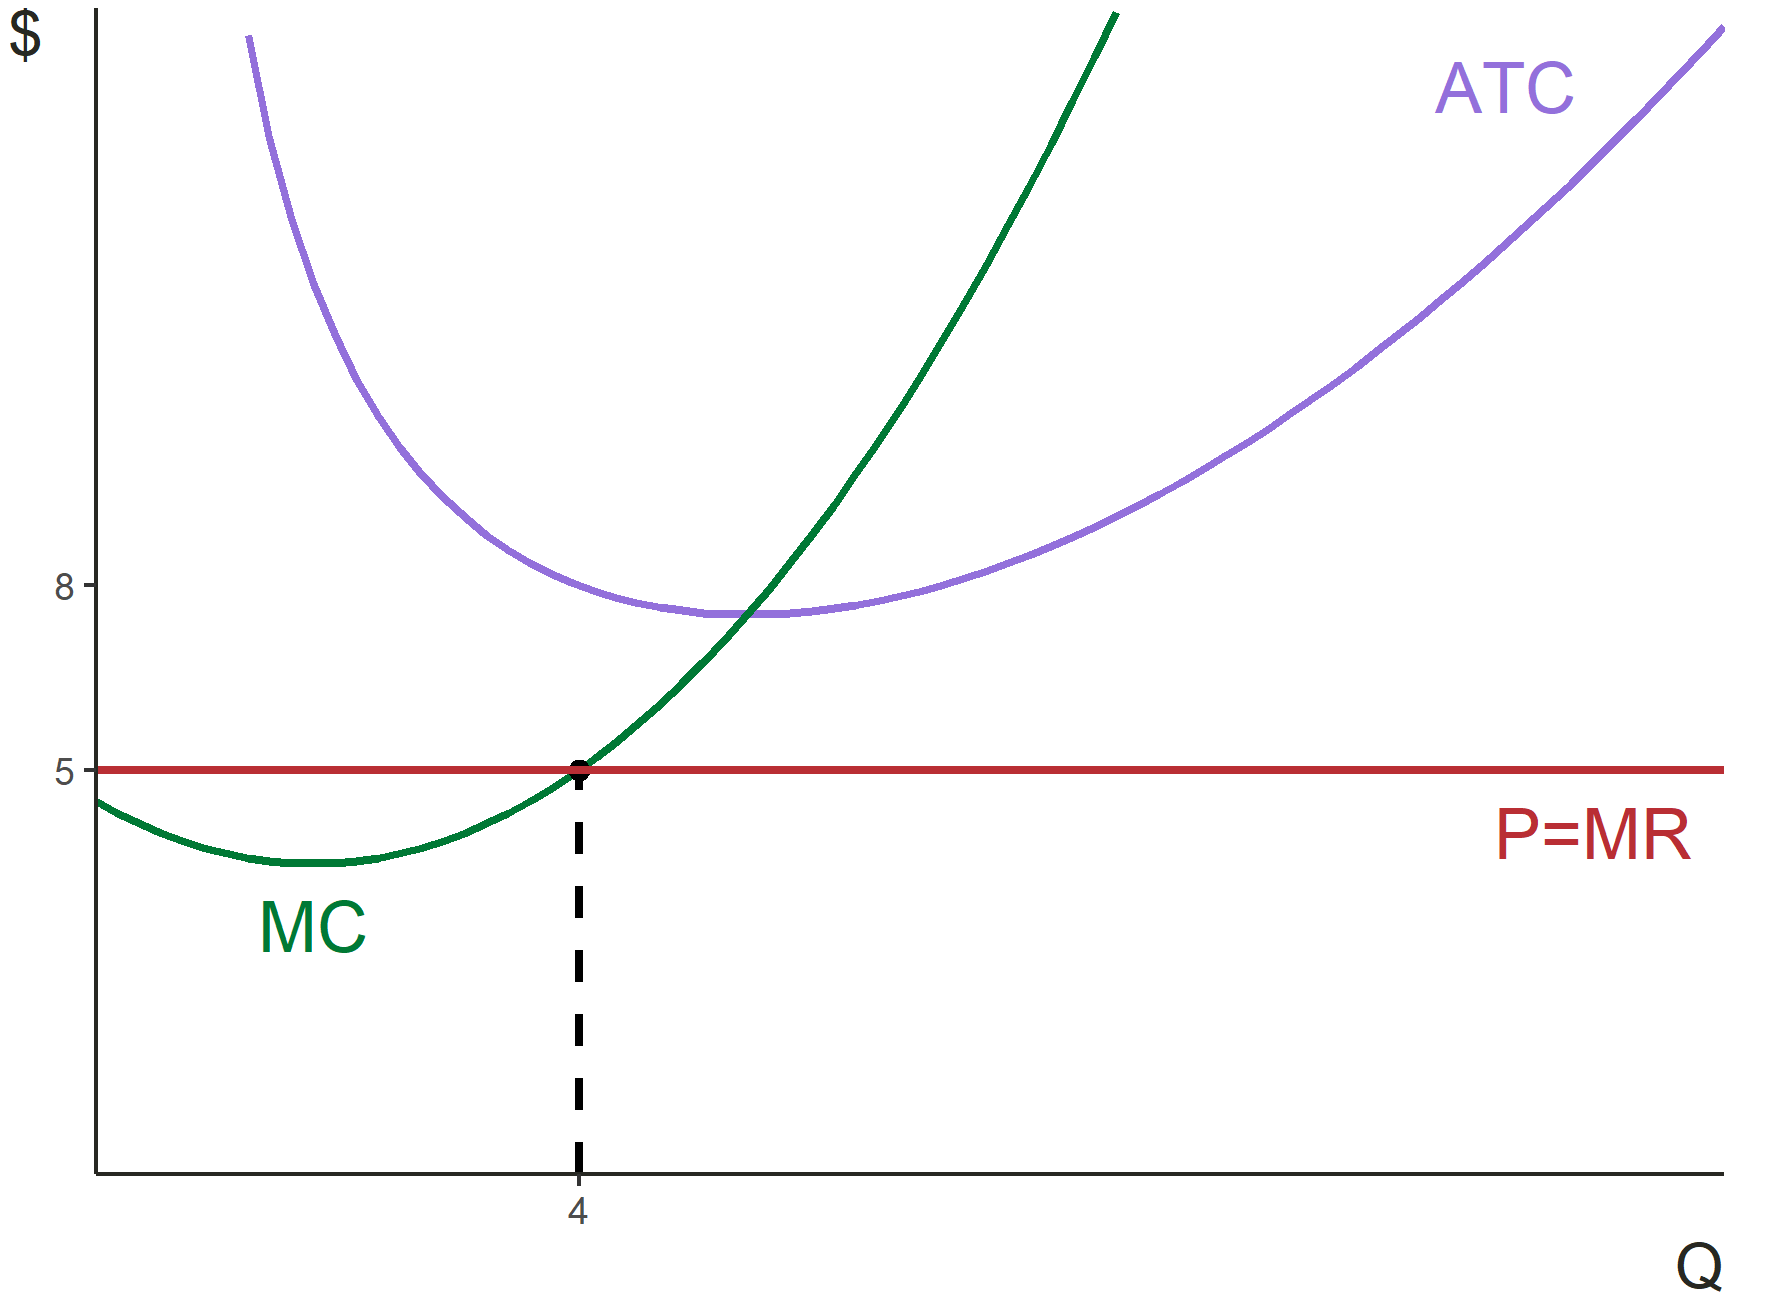
\includegraphics[width=8cm]{prod dec 3.png}
        \end{figure}
    \end{itemize}
\end{frame}

\begin{frame}{Visualizing Negative Profit for a PC Firm}
    \begin{itemize}[<+->]
        \item Specifically, we make $\pi=4(5-8)=-12$ 
        \begin{figure}
            \centering
            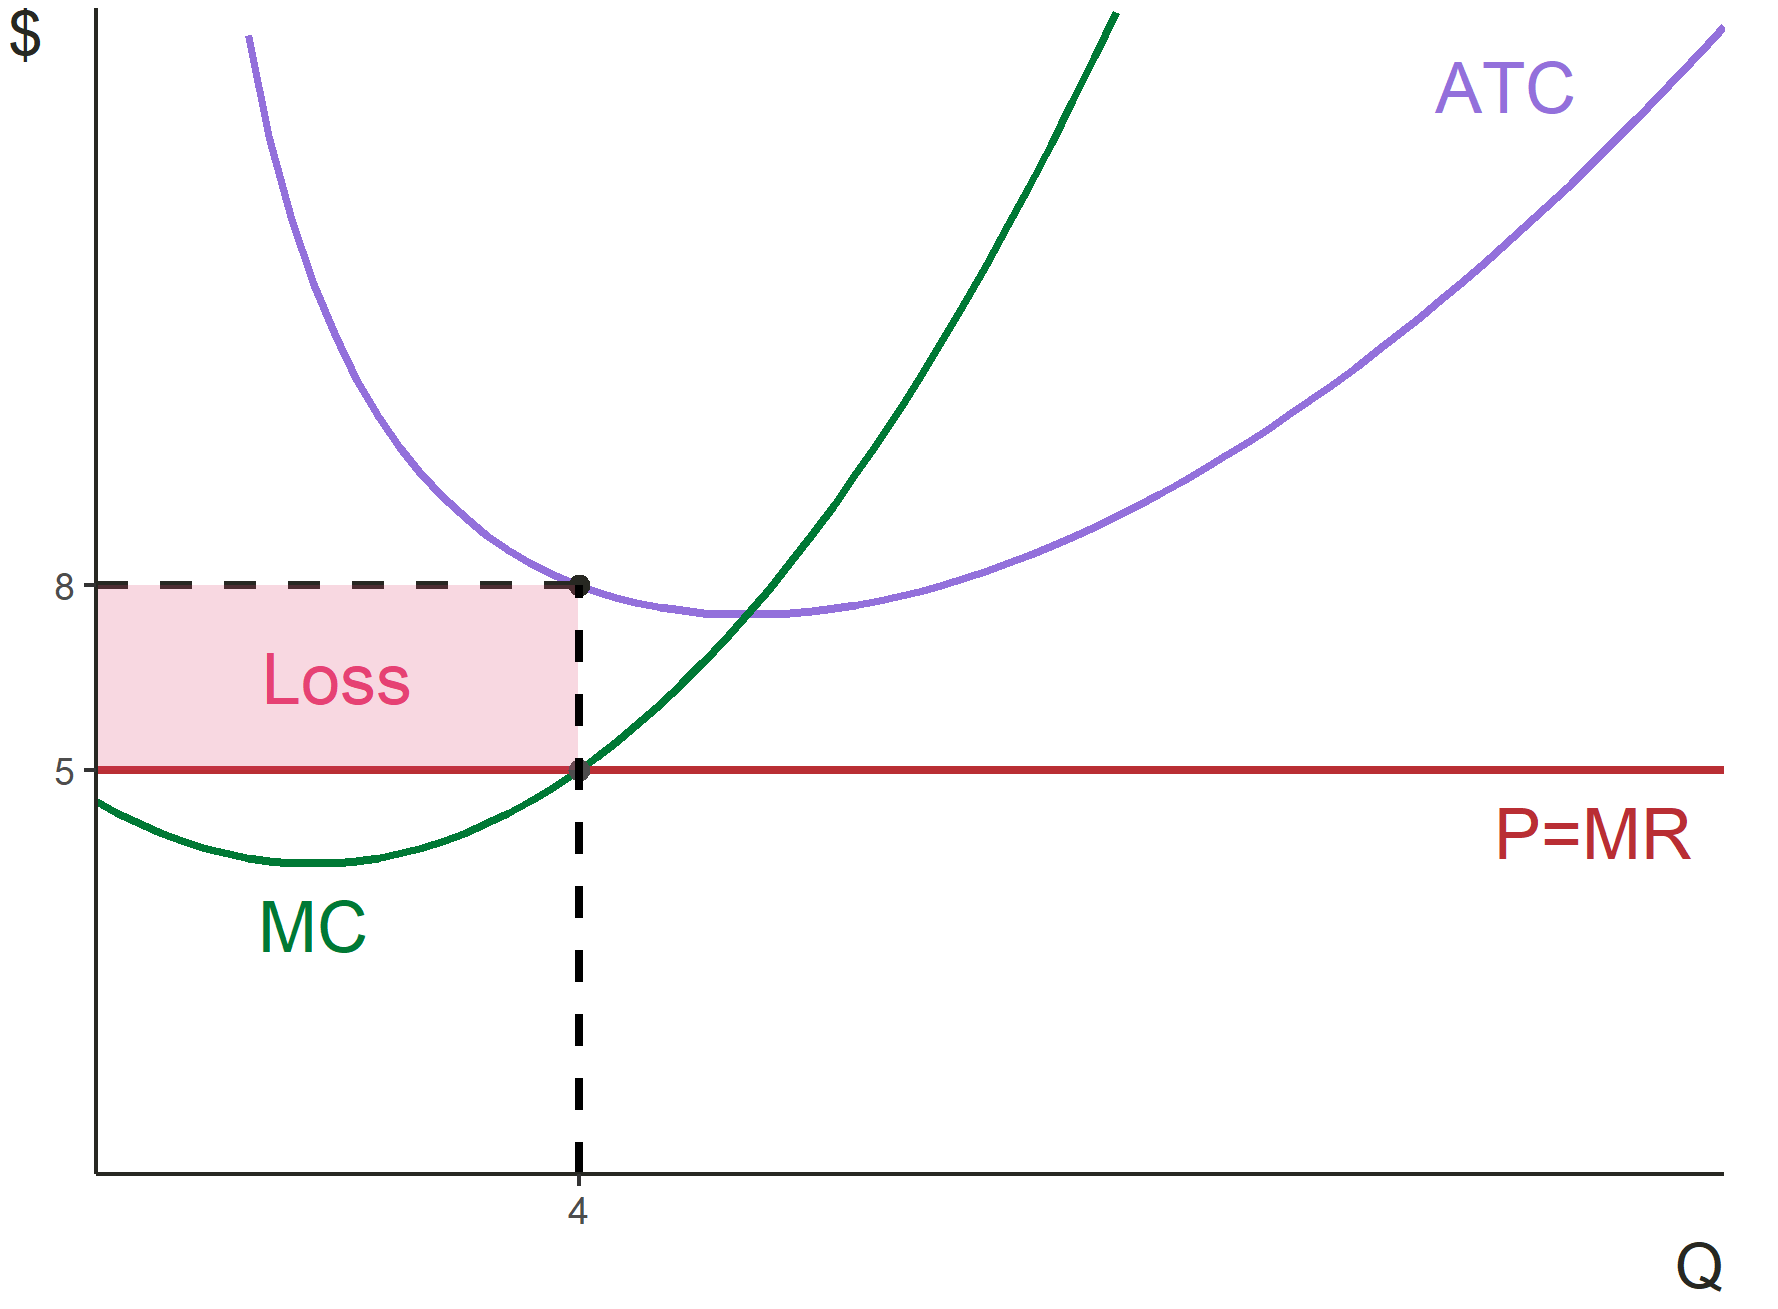
\includegraphics[width=8cm]{pmax3.png}
        \end{figure}
    \end{itemize}
\end{frame}

\begin{frame}{How the Book Derives Optimal Profit for the Firm}
    \begin{itemize}[<+->]
        \item The book carries this discussion a little differently than I have
        \begin{itemize}
            \item One result that the book points out\footnote{I don't know if we will find use for this} is that if we were to define \underline{average revenue} as $\frac{TR}{Q}$, then
            $$AR=\frac{PQ}{Q}=P$$
            \item Therefore, for \textit{any} firm, AR is equal to the price
        \end{itemize}
        \item They motivate the profit maximization of the firm using more table-thinking. I expect you to read this on your own (mainly 14-1b thru 14-2b, but all of chapter 14)
    \end{itemize}
\end{frame}

\end{document}